\chapter{Numerical simulations}

This chapter will cover the numerical simulation used to compare and analyse the behavior of two image restoration methods previously described: PIDSplit+ and AEM.

\section{Test-problems}

In the experiments, we used a set of test-problems, mainly from two categories: artificial and real problems.

\subsection{Simulated problems}

This class of problems consists in images in which Poisson noise is simulated by the \verb|imnoise| function, provided by the Matlab Image Processing Toolbox.

\subsubsection{LCR phantom}

The original image is an array  $256 \times 256$ consisting in three concentric circles of intensities 70, 135 and 200 respectively, enclosed by a square frame of intensity 10, all on a background of intensity 5 (LCR-1).

Several noise levels can be simulated multiplying such LCR phantom by a factor 10 (LCR-10) and 0.2 (LCR-0.2) and subsequently generating the corresponding noisy images.

\begin{figure}[H]
\begin{center}$
\begin{array}{cc}
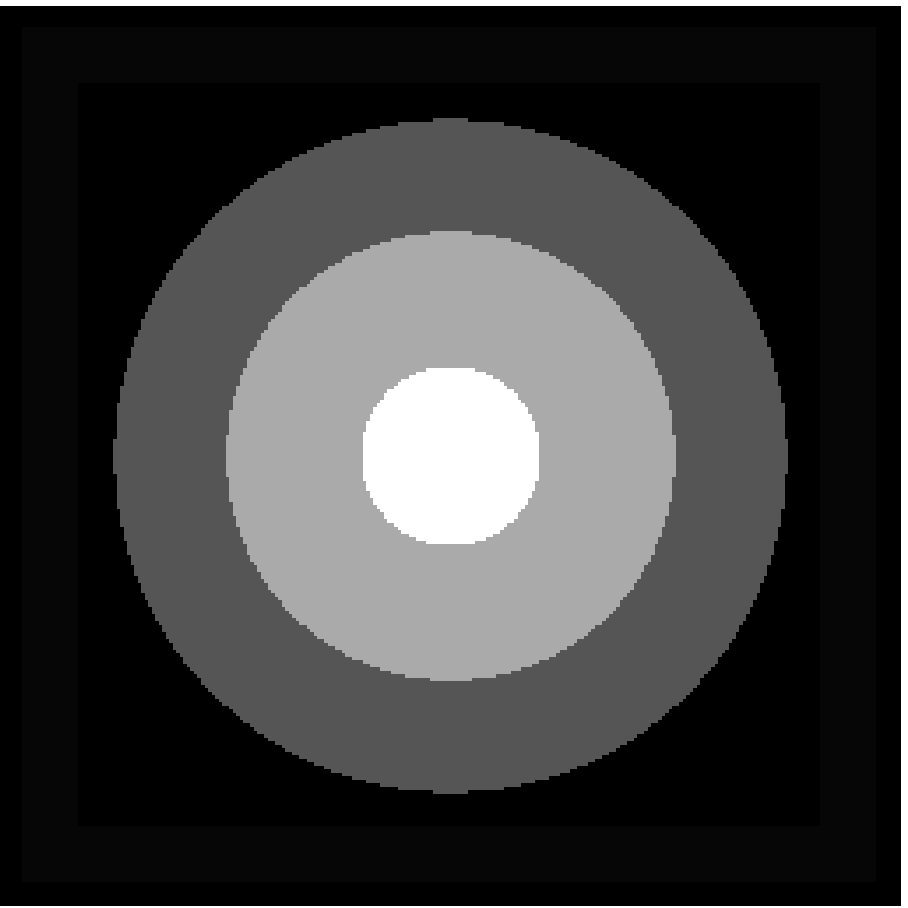
\includegraphics[width=6 cm]{img/circles} & 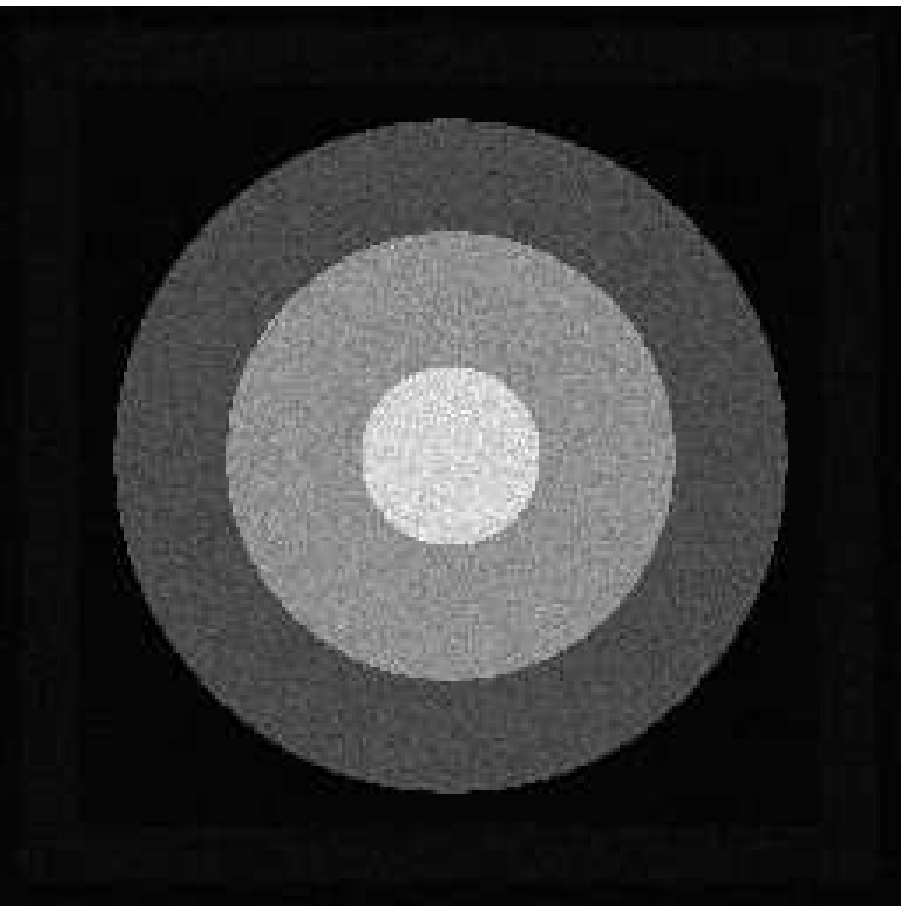
\includegraphics[width=6 cm]{img/circles_noisy}
\end{array}$
\end{center}
\caption{LCR-1: the original image and the noisy one}
\end{figure}

\begin{figure}[H]
\begin{center}$
\begin{array}{cc}
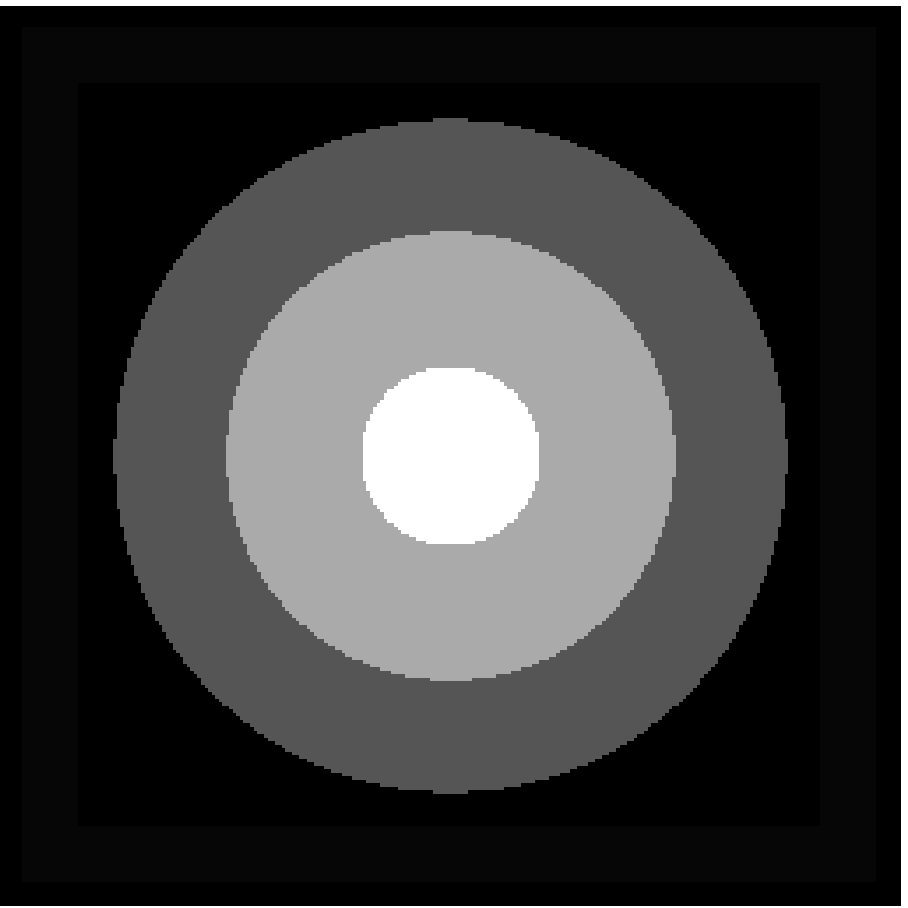
\includegraphics[width=6 cm]{img/circles_10} & 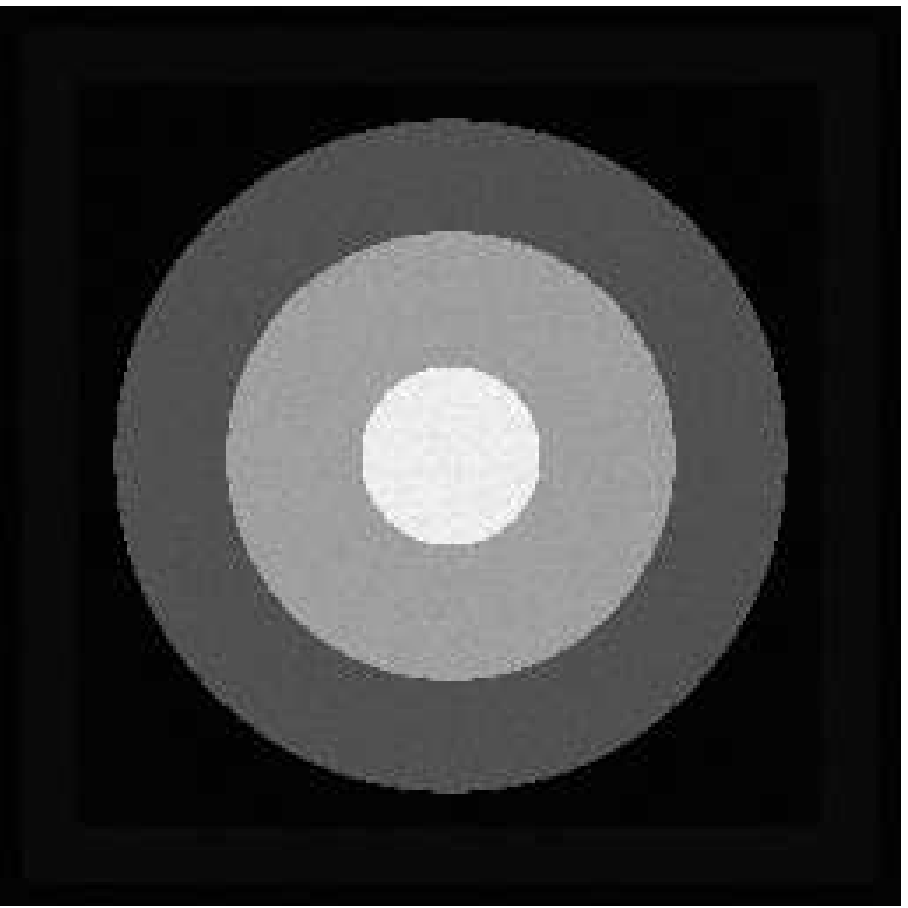
\includegraphics[width=6 cm]{img/circles_10_noisy}
\end{array}$
\end{center}
\caption{LCR-10: the original image and the noisy one}
\end{figure}

\begin{figure}[H]
\begin{center}$
\begin{array}{cc}
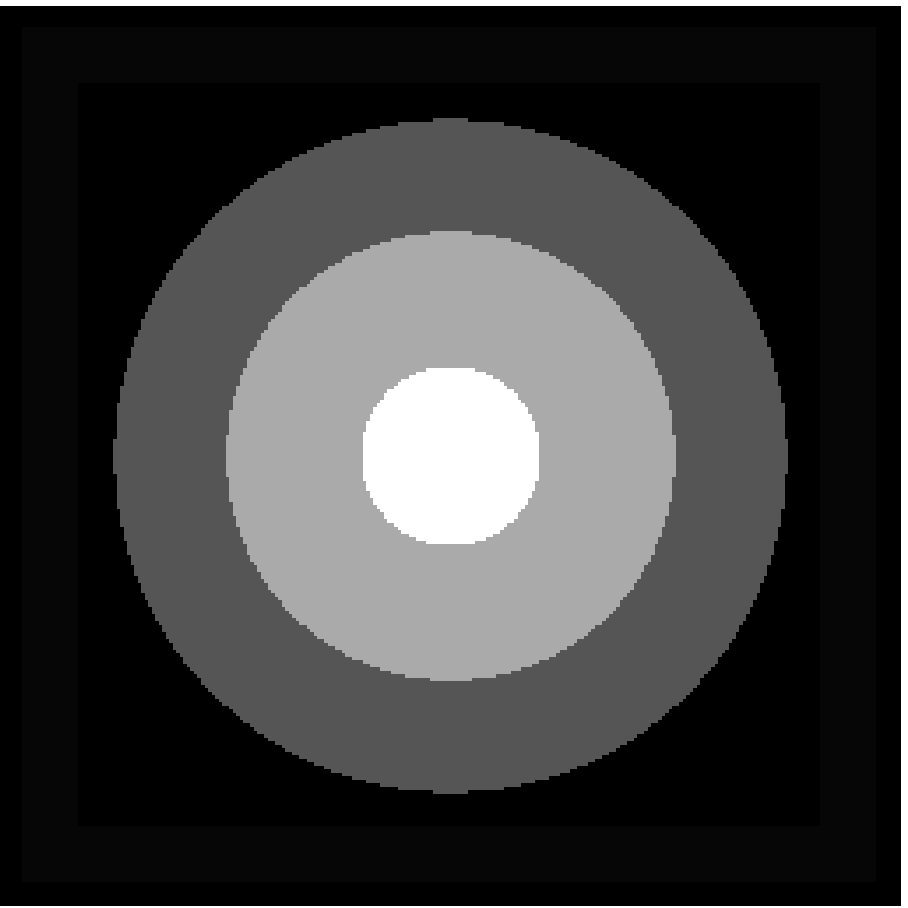
\includegraphics[width=6 cm]{img/circles_d5} & 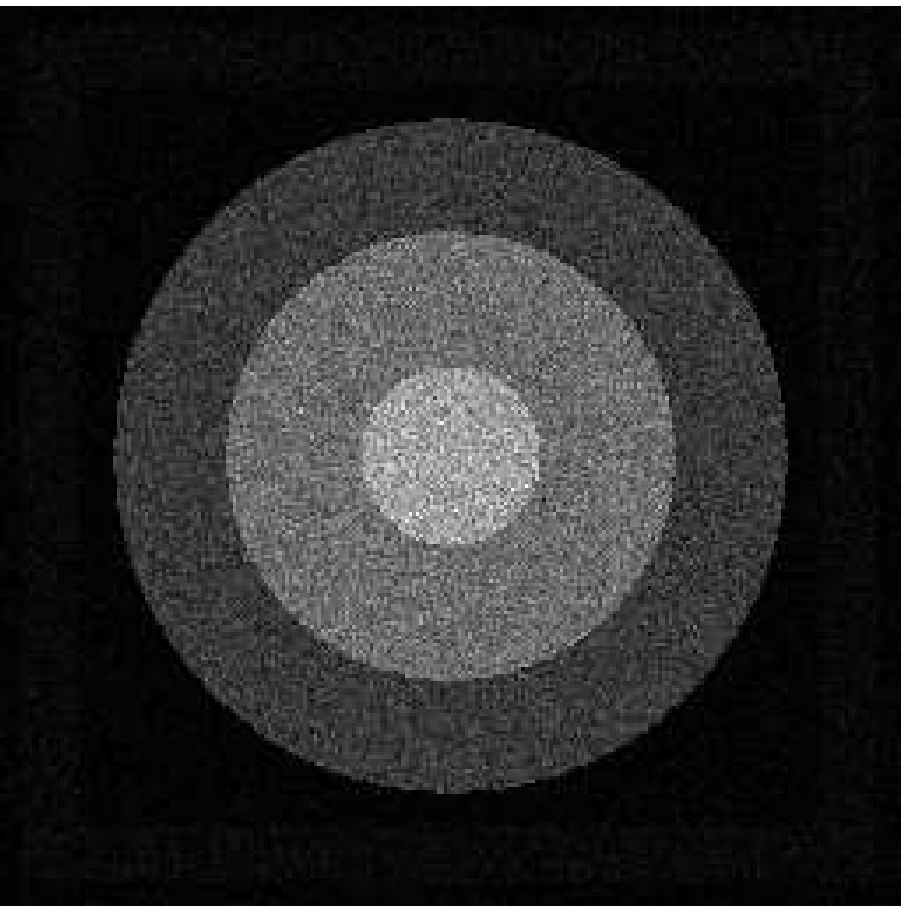
\includegraphics[width=6 cm]{img/circles_d5_noisy}
\end{array}$
\end{center}
\caption{LCR-0.2: the original image and the noisy one}
\end{figure}

\subsubsection{Airplane}
The original image is an array $256 \times 256$ depicting an aerial image of an airplane on a runway, with values in the range $[0,232]$.

\begin{figure}[H]
\begin{center}$
\begin{array}{cc}
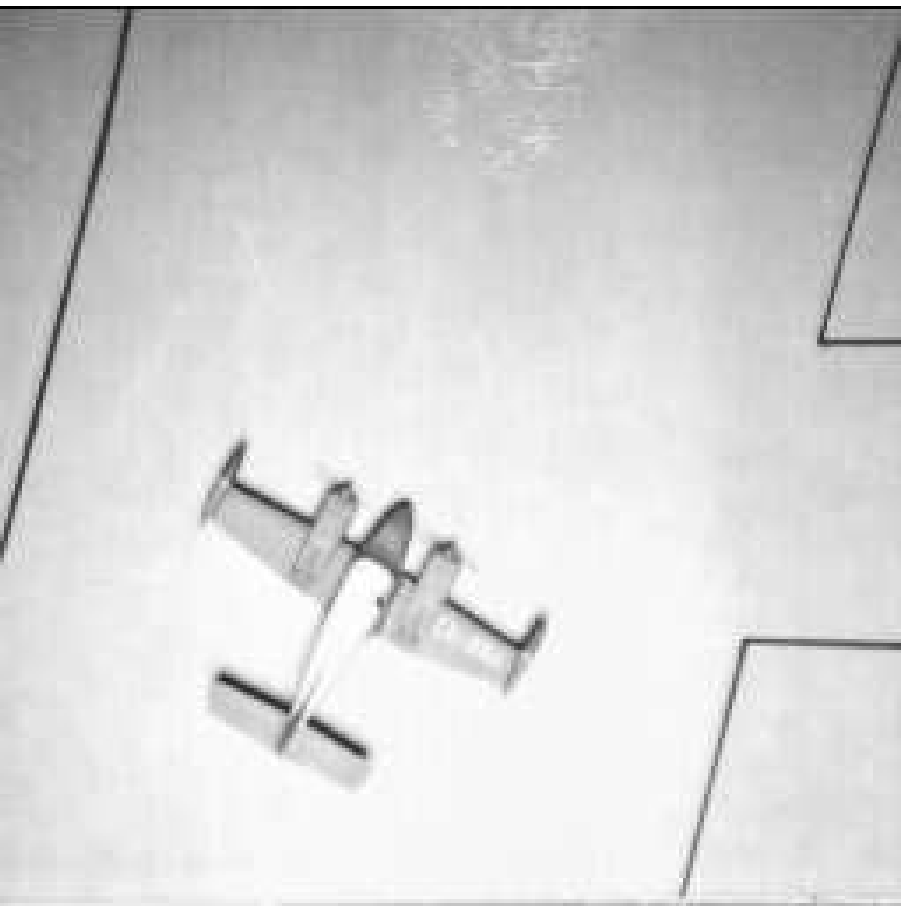
\includegraphics[width=6 cm]{img/airplane} & 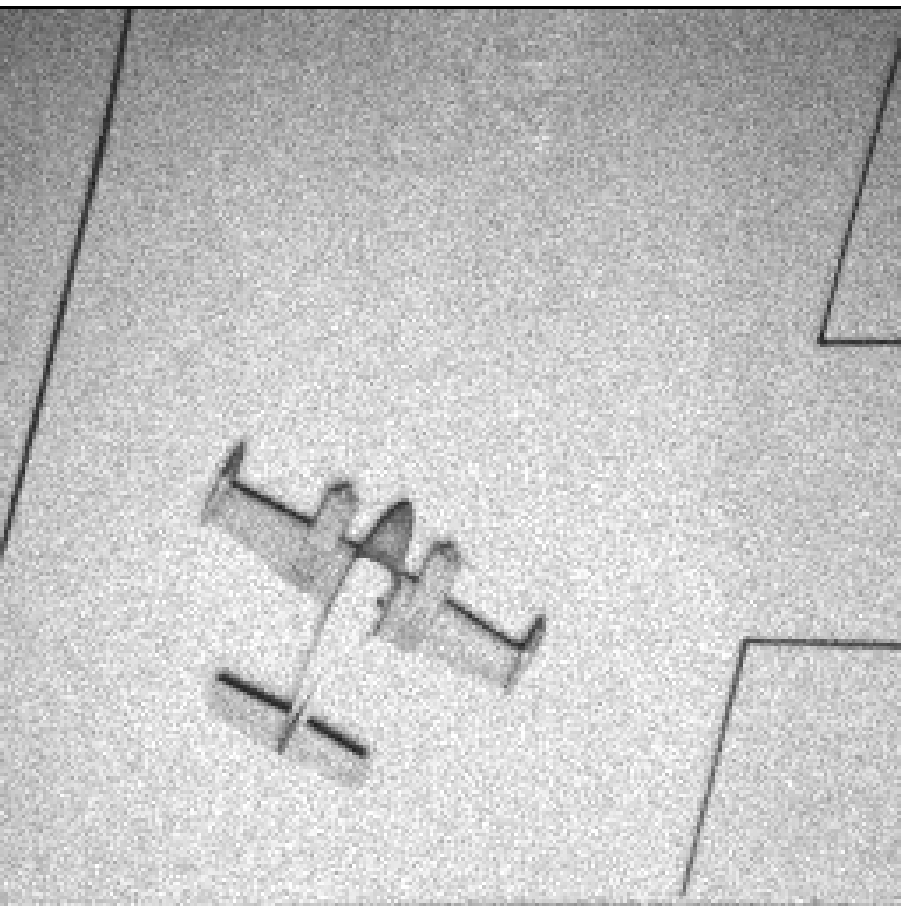
\includegraphics[width=6 cm]{img/airplane_noisy}
\end{array}$
\end{center}
\caption{Airplane: the original image and the noisy one}
\end{figure}


\subsubsection{Dental Radiography (DR)}

The original image is an array $512 \times 512$ with values in the range $[0,255]$.

\begin{figure}[H]
\begin{center}$
\begin{array}{cc}
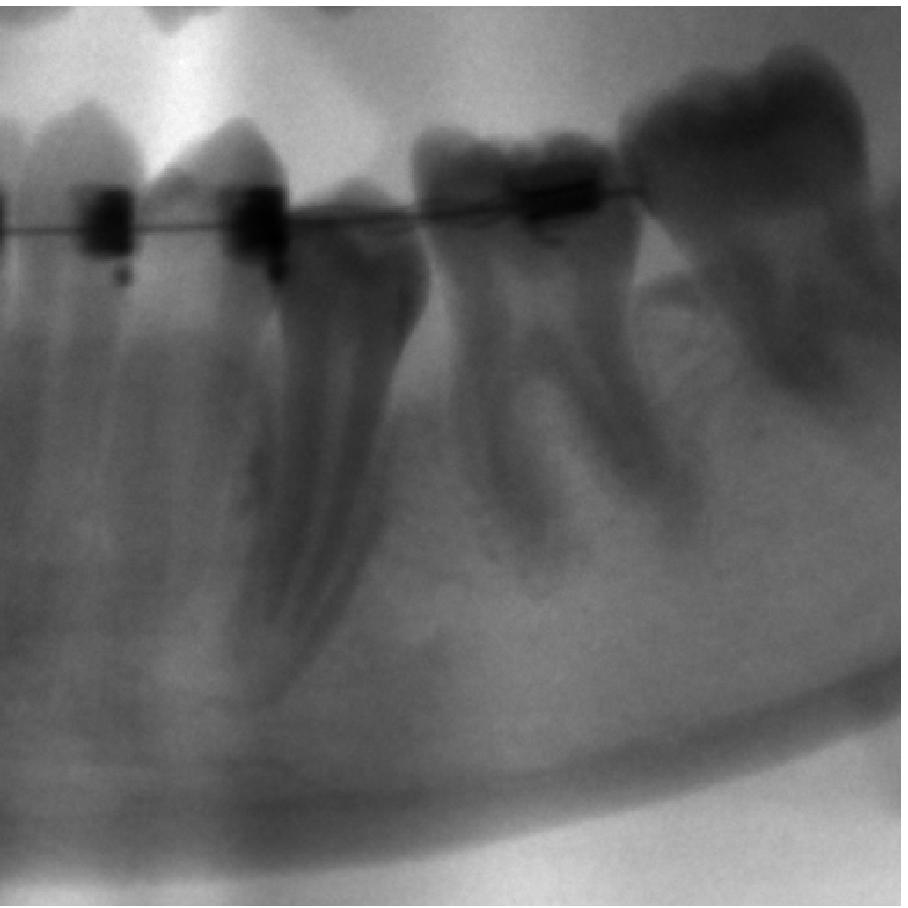
\includegraphics[width=6 cm]{img/Panoramica} & 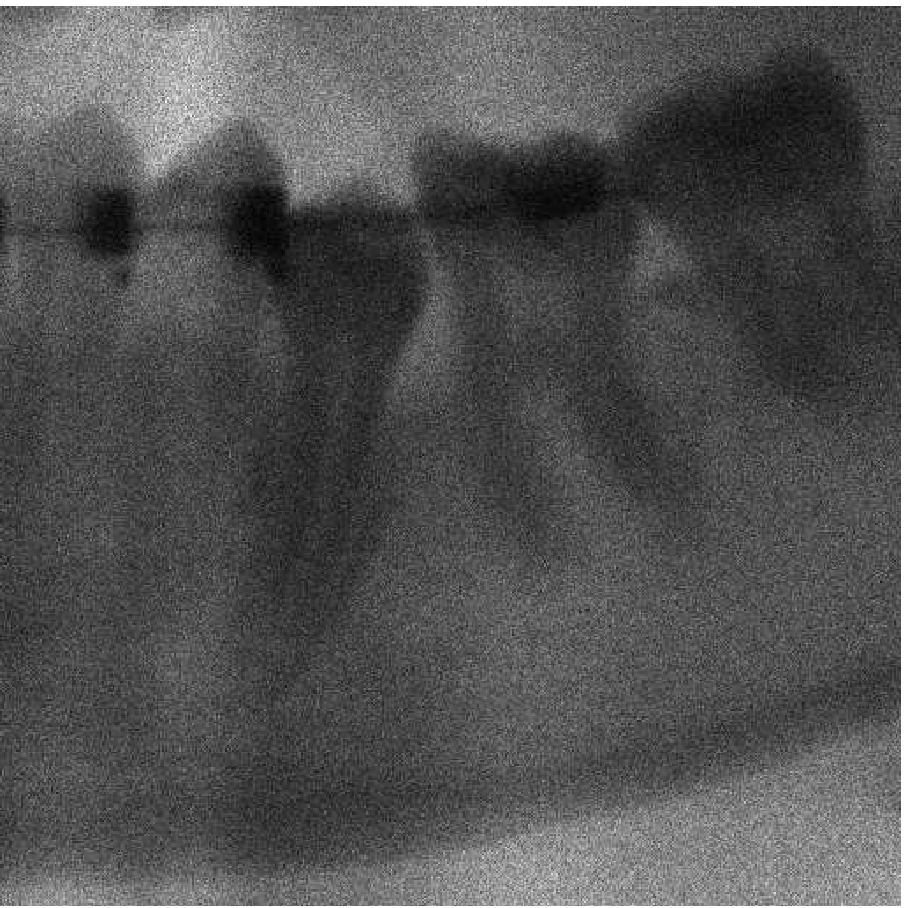
\includegraphics[width=6 cm]{img/Panoramica_noisy}
\end{array}$
\end{center}
\caption{DR: the original image and the noisy one}
\end{figure}

\subsection{Real-world problems}

As an example of problems that occurs in real world, we studied a number of images (\verb|Image11|, \verb|Image13|, \verb|Image22|, \verb|Image48|, \verb|Image49|, \verb|Image50|) from the project ``PRISMA''\footnote{See \url{http://www.unife.it/prisma}.} (optimizAtion Methods and Software for Inverse PRoblems) which represent dental radiographies affected by Poisson noise.

Every image is a ``negative'' array of $266 \times 266$ meaning that the level 4095 stands for 0 photon collected, whereas 0 stands for sensor saturation.

To obtain an image in which the gray level is linear with respect to the number of photon collected, the following transformation (with $X$ as the image array) has been used:

$$ Z = 4095 - X$$

An important difference between the simulated problems and these real ones, is that for the formers we had a noise-free image, while for the latters we do not. For this reason, a provided ``ground truth'' image has been used.

\begin{figure}[H]
\begin{center}
\includegraphics[width=6cm]{img/avg}
\end{center}
\caption{Ground truth.}
\end{figure}

\begin{figure}[H]
\begin{center}$
\begin{array}{cc}
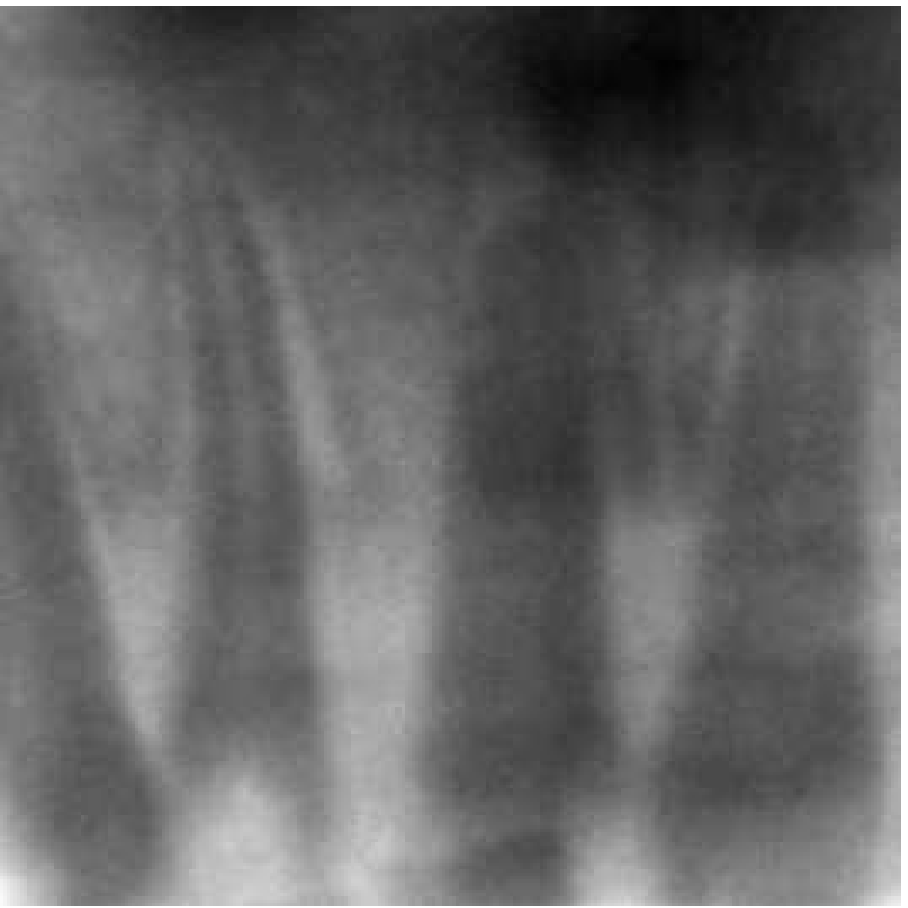
\includegraphics[width=6cm]{img/11}  & 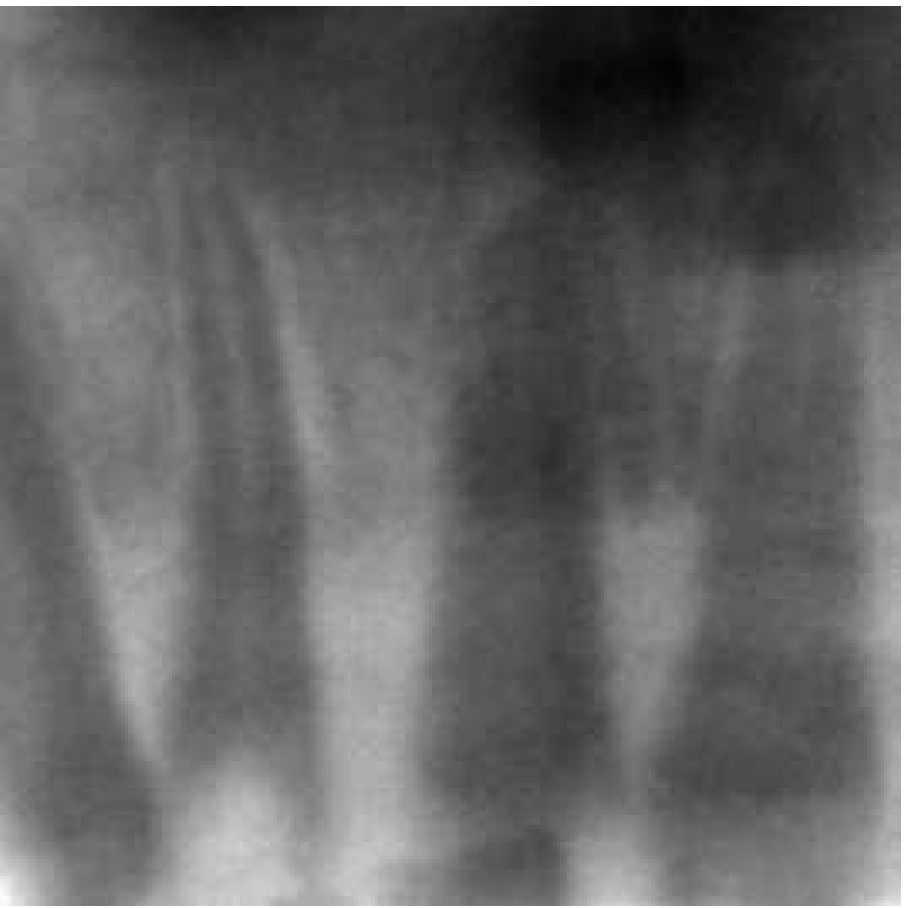
\includegraphics[width=6cm]{img/13}
\\
\mbox{Image11} & \mbox{Image 13}
\end{array}$
\end{center}
\end{figure}

\begin{figure}[H]
\begin{center}$
\begin{array}{cc}
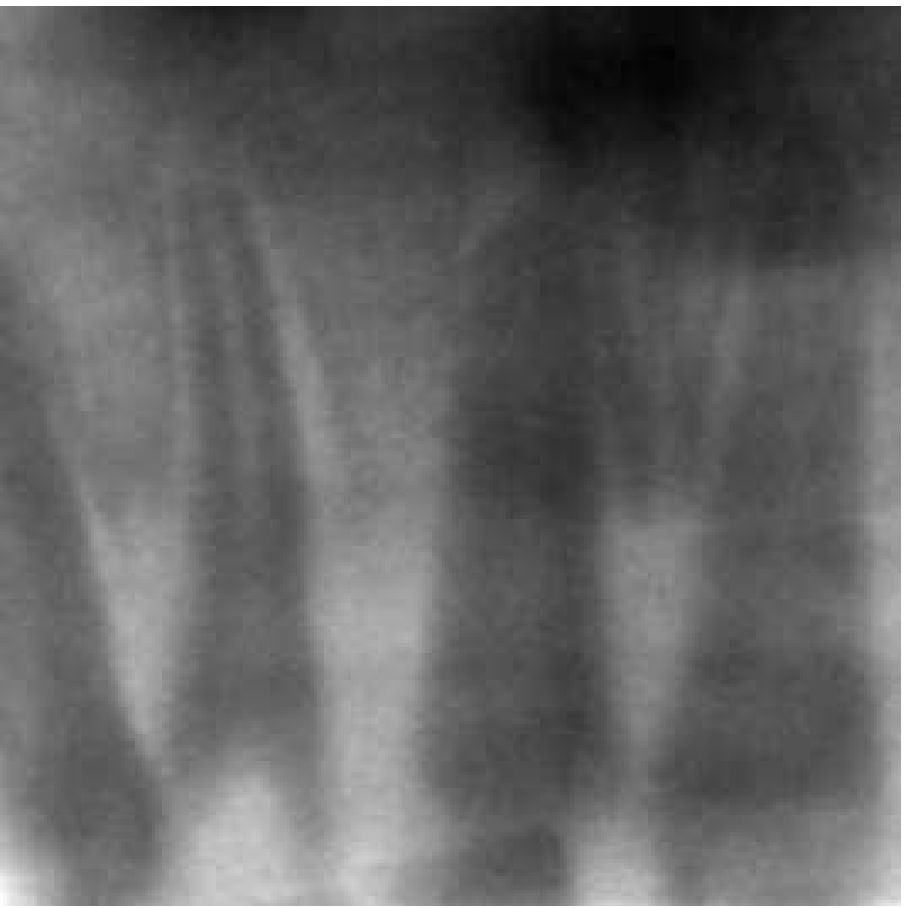
\includegraphics[width=6cm]{img/22}  & 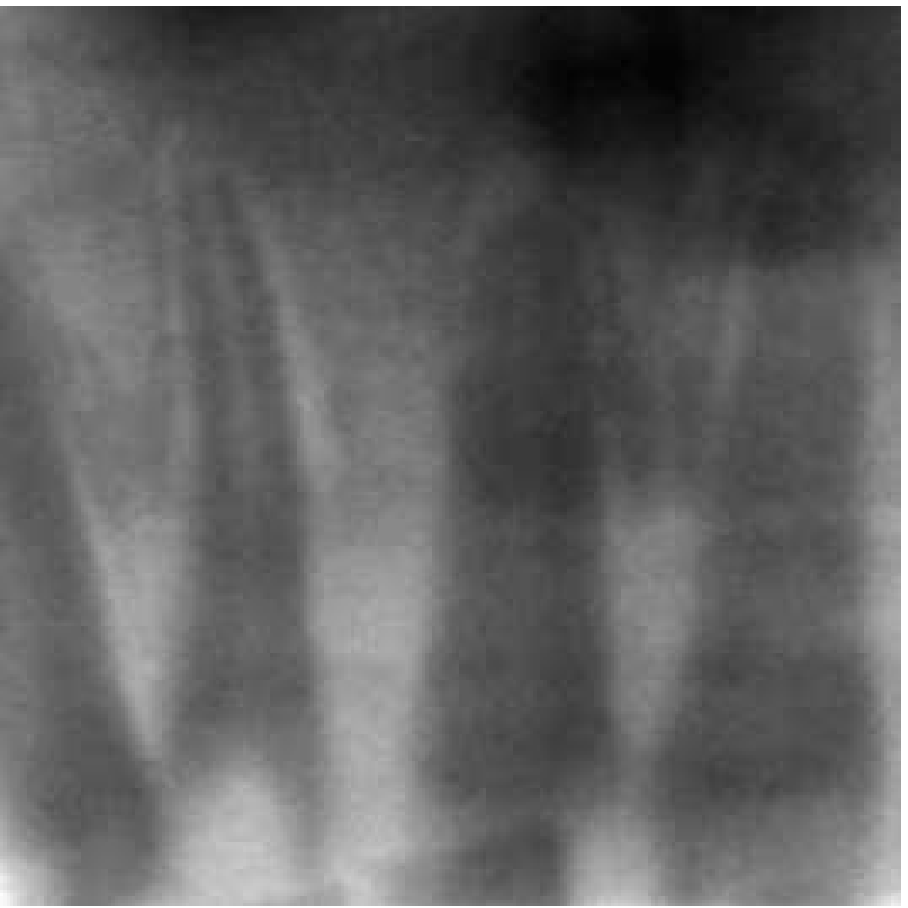
\includegraphics[width=6cm]{img/48}
\\
\mbox{Image22} & \mbox{Image 48}
\end{array}$
\end{center}
\end{figure}

\begin{figure}[H]
\begin{center}$
\begin{array}{cc}

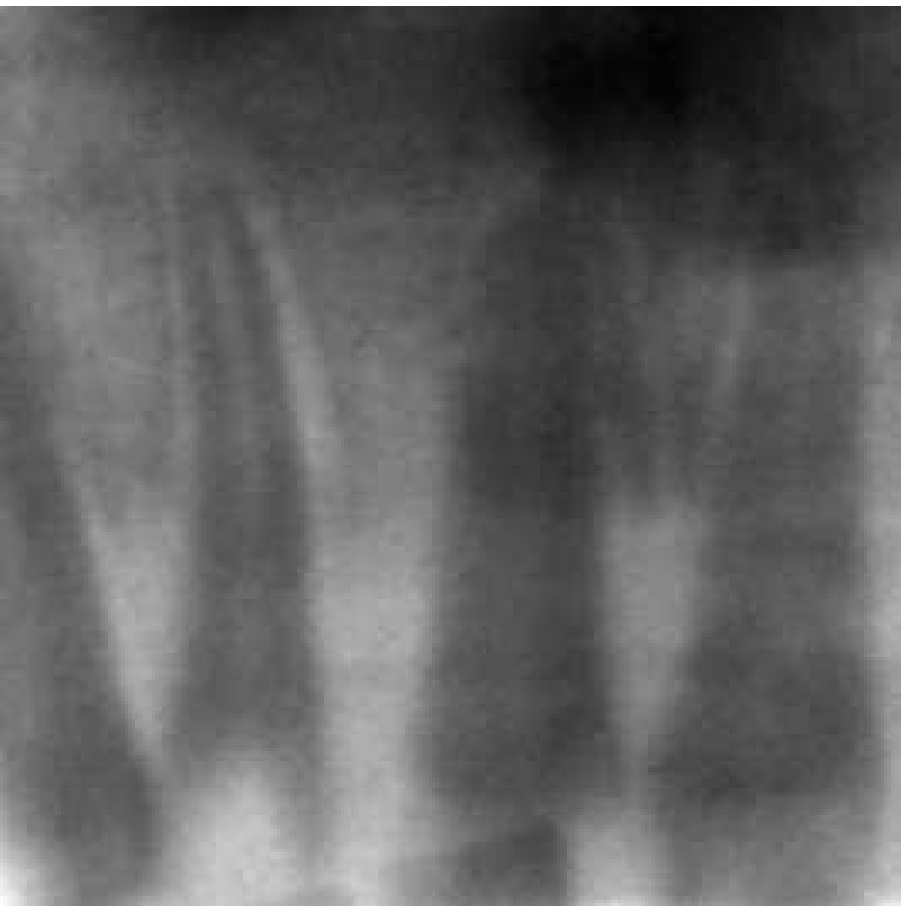
\includegraphics[width=6cm]{img/49}  & 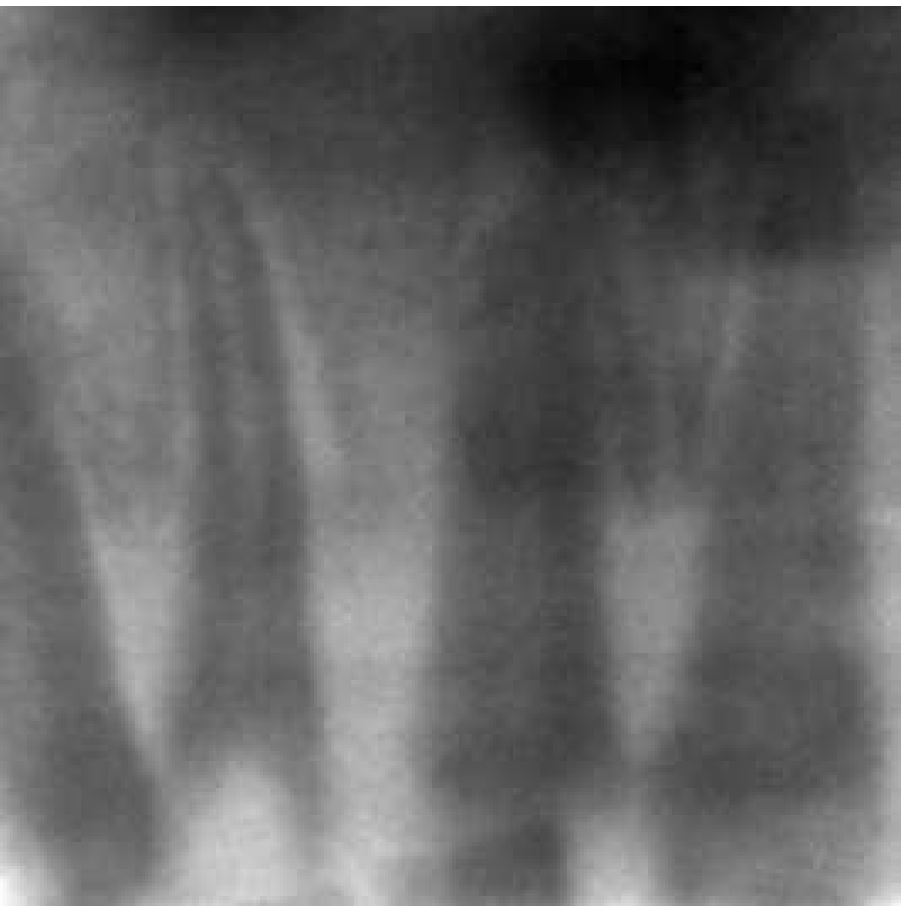
\includegraphics[width=6cm]{img/50}
\\
\mbox{Image49} & \mbox{Image 50}
\end{array}$
\end{center}
\end{figure}

\section{Numerical stability of AEM and PIDSplit+}

In the first set of experiments we compare the numerical behavior of the methods previously described, PIDSplit+ and AEM, on the five denoising problems LCR-1, LCR-10, LCR-0.2, Airplane, and DR.

To get the ideal solution $\tilde{x}$ of the minimization problem, we run AEM until 10000 iterations are reached.

Both the algorithms have been initialized with $x^{(0)} = max\{\eta,f\}$, where the maximum is meant component-wise, $\eta$ is the same as in \eqref{domain} and $f$ is the noisy image. The initial guess for the dual variable $y^{(0)}$ for AEM has been set to zero.

The values of $\beta$ used for each problem in \eqref{map}, as suggested in \citep{zanella}, are shown in the following table:

\begin{table}[H]
\begin{center}
\renewcommand*{\arraystretch}{1.4}
\begin{tabular}{m{1.8cm}|m{1cm}}
Problem & $\beta$ \\
\hline
LCR-1 & 0.25 \\
\hline
LCR-10 & 0.05 \\
\hline
LCR-0.2 & 0.575 \\
\hline
Airplane & 0.05 \\
\hline
DR & 0.27 \\
\end{tabular}
\caption{Values of $\beta$}
\end{center}
\end{table}

Since the value of $\gamma$ required by the PIDSplit+ algorithm is a user-supplied parameter which depends on the problem, we choose the values shown in the table below, along with the name used to refer to the PIDSplit+ algorithm with a particular value of $\gamma$.

\begin{table}[H]
\begin{center}
\renewcommand*{\arraystretch}{1.8}
\begin{tabular}{C{0.8cm}|C{1cm}}
$\gamma$ & Label \\
\hline
$50/\beta$ & PID50 \\
\hline
$5/\beta$ & PID5 \\
\hline
$1/\beta$ & PID1 \\
\hline
$0.5/\beta$ & PID05 \\
\end{tabular}
\caption{Values of $\gamma$ and the labels used.}
\end{center}
\end{table}

In order to evaluate the accuracy of the results and the effectiveness of the methods, in the following tables we report the iteration (\emph{iter}) and time ($t^{(iter)}$) in seconds required to reach a particular threshold of relative error, defined as

$$\epsilon^{(iter)} = \dfrac{\left|\left|x^{(iter)}-\tilde{x}\right|\right|_2}{\left|\left|\tilde{x}\right|\right|_2}$$

where $iter$ is the iteration number and $\tilde{x}$ is the approximate solution of the minimization problem, as described previously.

Furthermore, we define the relative reconstruction error:

$$e^{(iter)} = \dfrac{\left|\left|x^{(iter)}-x^*\right|\right|_2}{\left|\left|x^*\right|\right|_2}$$

where $x^*$ is the original, noise-free, image.

An empty cell in the following tables indicates that the particular error threshold $\epsilon$ has not been reached in 3000 iterations.

\begin{table}[H]
\begin{center}
\renewcommand*{\arraystretch}{1.5}
\begin{tabular}{|C{1.2cm}|C{0.9cm}|C{0.9cm}|C{1.5cm}|C{0.9cm}|C{0.9cm}|C{1.5cm}|}\hline

Method & \multicolumn{3}{c|} {$\epsilon = 10^{-2}$}  & \multicolumn{3}{c|} {$\epsilon = 10^{-4}$} \\ \cline{2-7}
     & \emph{iter} & $t^{(iter)}$ & $e^{(iter)}$ & \emph{iter} & $t^{(iter)}$  & $e^{(iter)}$  \\ \hline
AEM & 64 & 3.45 & 0.0230578 & 605 & 29.91 & 0.0249536   \\ \hline
PID50 & 65 & 3.47 & 0.0277052 & & &  \\ \hline
PID5 & 27 & 1.42 & 0.0250464 & 1023 & 57.9 & 0.0249536    \\ \hline
PID1 & 82 & 4.43 & 0.022816 & 594 & 33.43 & 0.0249649 \\ \hline
PID05 & 158 & 9.17 & 0.0226965 & 1183 & 66.91 & 0.0249641  \\ \hline
     & \multicolumn{3}{c|} {$\epsilon = 10^{-5}$}  & \multicolumn{3}{c|} {$\epsilon = 5\cdot 10^{-6}$}  \\ \cline{2-7}
     & \emph{iter} & $t^{(iter)}$  & $e^{(iter)}$ & \emph{iter} & $t^{(iter)}$  & $e^{(iter)}$ \\ \hline
AEM   & 1943 & 96.67 & 0.0249837 & & &  \\ \hline
PID50 & & & & & &  \\ \hline
PID5  & & & & & &  \\ \hline
PID1  & 1029 & 58.08 & 0.0249835 & 1478 & 83.33 & 0.0249836  \\ \hline
PID05 & 1932 & 109.24 & 0.0249832 & 2186 & 124.34 & 0.249834 \\ \hline
\end{tabular}
\caption{Results for LCR-1}
\label{tab:err2}
\end{center}
\end{table}

\begin{table}[H]
\begin{center}
\renewcommand*{\arraystretch}{1.5}
\begin{tabular}{|C{1.2cm}|C{1cm}|C{2.2cm}|C{1.5cm}|}\hline
Method & $t^{(3000)}$ & $\epsilon^{(3000)}$ & $e^{(3000)}$ \\ \hline
AEM &  149.91 & $6.3934 \cdot 10^{-6}$ & 0.0249836 \\ \hline
PID50 &  167.23 & $3.30784 \cdot 10^{-4}$ & 0.0249921 \\ \hline
PID5 &  170.81 & $1.86697 \cdot 10^{-5}$ & 0.0249839 \\ \hline
PID1 &  169.24 & $2.40734 \cdot 10^{-6}$ & 0.0249835 \\ \hline
PID05 &  169.9 & $1.0246 \cdot 10^{-6}$ & 0.0249835 \\ \hline
\end{tabular}
\caption{Results for LCR-1 after 3000 iterations.}
\end{center}
\end{table}

%% inizio lcr-10

\begin{table}[H]
\begin{center}
\renewcommand*{\arraystretch}{1.5}
\begin{tabular}{|C{1.2cm}|C{0.9cm}|C{0.9cm}|C{1.7cm}|C{0.9cm}|C{0.9cm}|C{1.7cm}|}\hline
Method & \multicolumn{3}{c|} {$\epsilon = 10^{-2}$}  & \multicolumn{3}{c|} {$\epsilon = 10^{-4}$} \\ \cline{2-7}
     & \emph{iter} & $t^{(iter)}$  & $e^{(iter)}$ & \emph{iter} & $t^{(iter)}$  & $e^{(iter)}$  \\ \hline
AEM & 92 & 4.65 & 0.0118767 & 816 & 40.9 & 0.00835666   \\ \hline
PID50 & 5 & 0.22 & 0.0110561 & 540 &  30.13 & 0.00838595  \\ \hline
PID5 & 24 & 1.24 & 0.00119889 & 320 & 17.94 & 0.00833781    \\ \hline
PID1 & 116 & 6.39 & 0.0119236 & 1592 & 96.69 & 0.00833768 \\\hline
     & \multicolumn{3}{c|} {$\epsilon = 10^{-5}$}  & \multicolumn{3}{c|} {$\epsilon = 5\cdot 10^{-6}$}  \\ \cline{2-7}
     & \emph{iter} & $t^{(iter)}$  & $e^{(iter)}$ & \emph{iter} & $t^{(iter)}$  & $e^{(iter)}$ \\ \hline
AEM   & 1360 & 66.87 & 0.00838057 & 1531 & 74.92 & 0.00838169  \\ \hline
PID50 & 2622 & 146.63 & 0.00838286 & & &  \\ \hline
PID5  &  558 & 31.19 & 0.00837926 &  654 &  36.6 & 0.00838144  \\ \hline
PID1  & 2731 & 153.58 & 0.00837883 & & &  \\ \hline
\end{tabular}
\caption{Results for LCR-10}
\end{center}
\end{table}

\begin{table}[H]
\begin{center}
\renewcommand*{\arraystretch}{1.5}
\begin{tabular}{|C{1.2cm}|C{1cm}|C{2.2cm}|C{1.7cm}|}\hline
Method & $t^{(3000)}$ & $\epsilon^{(3000)}$ & $e^{(3000)}$ \\ \hline
AEM &  143.01 & $2.23187 \cdot 10^{-7}$ & 0.00838268 \\ \hline
PID50 &  167.66 & $8.25419 \cdot 10^{-6}$ & 0.00838283 \\ \hline
PID5 &  169.4 & $7.34523 \cdot 10^{-7}$ & 0.00838268 \\ \hline
PID1 &  169.15 & $5.8626 \cdot 10^{-6}$ & 0.00832767 \\ \hline
\end{tabular}
\caption{Results for LCR-10 after 3000 iterations.}
\end{center}
\end{table}

%% inizio lcr-0.2

\begin{table}[H]
\begin{center}
\renewcommand*{\arraystretch}{1.5}
\begin{tabular}{|C{1.2cm}|C{0.9cm}|C{0.9cm}|C{1.7cm}|C{0.9cm}|C{0.9cm}|C{1.7cm}|}\hline


Method & \multicolumn{3}{c|} {$\epsilon = 10^{-2}$}  & \multicolumn{3}{c|} {$\epsilon = 10^{-4}$} \\ \cline{2-7}
     & \emph{iter} & $t^{(iter)}$  & $e^{(iter)}$ & \emph{iter} & $t^{(iter)}$  & $e^{(iter)}$  \\ \hline
AEM & 102 & 5.97 & 0.0441267 & 2104 & 113.06 & 0.0447745   \\ \hline
PID50 & 478 & 25.79 & 0.0465756 &  &  &  \\ \hline
PID5 & 60 & 3.04 & 0.0466034 & & &    \\ \hline
PID1 & 68 & 3.76 & 0.0438891 & 696 & 37.92 & 0.0447745 \\\hline
PID05 & 119 & 6.50 & 0.0432181 & 606 & 33.01 & 0.0447726 \\\hline
     & \multicolumn{3}{c|} {$\epsilon = 10^{-5}$}  & \multicolumn{3}{c|} {$\epsilon = 5\cdot 10^{-6}$}  \\ \cline{2-7}
     & \emph{iter} & $t^{(iter)}$  & $e^{(iter)}$ & \emph{iter} & $t^{(iter)}$  & $e^{(iter)}$ \\ \hline
AEM   & & & & & &  \\ \hline
PID50 & & & & & &  \\ \hline
PID5  & & & & & & \\ \hline
PID1  & 1418 & 77.80 & 0.044773 & 1591 & 87.5 & 0.047729 \\ \hline
PID05  & & & & & & \\ \hline
\end{tabular}
\caption{Results for LCR-0.2}
\end{center}
\end{table}

\begin{table}[H]
\begin{center}
\renewcommand*{\arraystretch}{1.5}
\begin{tabular}{|C{1.2cm}|C{1cm}|C{2.2cm}|C{1.7cm}|}\hline
Method & $t^{(3000)}$ & $\epsilon^{(3000)}$ & $e^{(3000)}$ \\ \hline
AEM &  160.72 & $4.42311 \cdot 10^{-5}$ & 0.0447735 \\ \hline
PID50 &  164.51 & $1.00901 \cdot 10^{-3}$ & 0.0448293 \\ \hline
PID5 &  165.22 & $1.34896 \cdot 10^{-4}$ & 0.0447752 \\ \hline
PID1 &  164.91 & $1.80577 \cdot 10^{-5}$ & 0.0447724 \\ \hline
PID05 &  164.95 & $2.79695 \cdot 10^{-5}$ & 0.0447722 \\ \hline
\end{tabular}
\caption{Results for LCR-0.2 after 3000 iterations.}
\end{center}
\end{table}

%% inizio airplane

\begin{table}[H]
\begin{center}
\renewcommand*{\arraystretch}{1.5}
\begin{tabular}{|C{1.2cm}|C{0.9cm}|C{0.9cm}|C{1.7cm}|C{0.9cm}|C{0.9cm}|C{1.7cm}|}\hline


Method & \multicolumn{3}{c|} {$\epsilon = 10^{-2}$}  & \multicolumn{3}{c|} {$\epsilon = 10^{-4}$} \\ \cline{2-7}
     & \emph{iter} & $t^{(iter)}$  & $e^{(iter)}$ & \emph{iter} & $t^{(iter)}$  & $e^{(iter)}$  \\ \hline
AEM & 68 & 3.32 & 0.0258942 & 192 & 9.02 & 0.0214011   \\ \hline
PID50 & 7 & 0.33 & 0.0227146 & 451 & 25.82  & 0.0213743 \\ \hline
PID5 & 18 & 0.96 & 0.0252871 & 75 & 4.23 & 0.0213782   \\ \hline
PID1 & 82 & 4.53 & 0.0258994 & 324 & 17.98 & 0.0213914 \\ \hline
PID05 & 163 & 9.06 & 0.0258684 & 646 & 36.93 & 0.0213913 \\ \hline
     & \multicolumn{3}{c|} {$\epsilon = 10^{-5}$}  & \multicolumn{3}{c|} {$\epsilon = 5\cdot 10^{-6}$}  \\ \cline{2-7}
     & \emph{iter} & $t^{(iter)}$  & $e^{(iter)}$ & \emph{iter} & $t^{(iter)}$  & $e^{(iter)}$ \\ \hline
AEM   & 266 & 12.86 & 0.0213756 & 350 & 17.03 & 0.0213742  \\ \hline
PID50 & & & & & &  \\ \hline
PID5  & 362 & 20.63 & 0.0213741 & 679 & 38.41 & 0.0213742 \\ \hline
PID1  & 481 & 26.78 & 0.0213754 & 534 & 30.02 & 0.0213748 \\ \hline
PID05 & 956 & 54.98 & 0.0213754 & 1056 & 60.53 & 0.0213748 \\ \hline
\end{tabular}
\caption{Results for Airplane}
\end{center}
\end{table}

\begin{table}[H]
\begin{center}
\renewcommand*{\arraystretch}{1.5}
\begin{tabular}{|C{1.2cm}|C{1cm}|C{2.2cm}|C{1.7cm}|}\hline
Method & $t^{(3000)}$ & $\epsilon^{(3000)}$ & $e^{(3000)}$ \\ \hline
AEM &  148.21 & $4.66582 \cdot 10^{-7}$ & 0.0213742 \\ \hline
PID50 &  172.8 & $1.07853 \cdot 10^{-5}$ & 0.0213741 \\ \hline
PID5 &  169.26 & $1.01562 \cdot 10^{-6}$ & 0.0213742 \\ \hline
PID1 &  169.1 & $1.97154 \cdot 10^{-7}$ & 0.0213742 \\ \hline
PID05 &  171.54 & $9.10447 \cdot 10^{-8}$ & 0.0213742 \\ \hline
\end{tabular}
\caption{Results for Airplane after 3000 iterations.}
\end{center}
\end{table}

%% inizio DR

\begin{table}[H]
\begin{center}
\renewcommand*{\arraystretch}{1.5}
\begin{tabular}{|C{1.2cm}|C{0.9cm}|C{0.9cm}|C{1.7cm}|C{0.9cm}|C{0.9cm}|C{1.7cm}|}\hline


Method & \multicolumn{3}{c|} {$\epsilon = 10^{-2}$}  & \multicolumn{3}{c|} {$\epsilon = 10^{-4}$} \\ \cline{2-7}
     & \emph{iter} & $t^{(iter)}$  & $e^{(iter)}$ & \emph{iter} & $t^{(iter)}$  & $e^{(iter)}$  \\ \hline
AEM & 43 & 8.24 & 0.0275251 & 481 & 93.32 & 0.0296553   \\ \hline
PID50 & 91 & 17.86 & 0.0277751 &  &  &  \\ \hline
PID5 & 19 & 3.53 & 0.0281259 & 921 & 195.09 & 0.0296544    \\ \hline
PID1 & 47 & 9.91 & 0.0288035 & 234 & 49.92 & 0.0296558 \\\hline
PID05 & 90 & 19.26 & 0.0291545 & 378 & 80.88 & 0.0296571 \\\hline
     & \multicolumn{3}{c|} {$\epsilon = 10^{-5}$}  & \multicolumn{3}{c|} {$\epsilon = 5\cdot 10^{-6}$}  \\ \cline{2-7}
     & \emph{iter} & $t^{(iter)}$  & $e^{(iter)}$ & \emph{iter} & $t^{(iter)}$  & $e^{(iter)}$ \\ \hline
AEM   & & & & & &  \\ \hline
PID50 & & & & & &  \\ \hline
PID5  & & & & & & \\ \hline
PID1  & 1361 & 291.52 & 0.0296611 & 2567 & 549.45 & 0.0296614 \\ \hline
PID05 & 726 & 154.72 & 0.0296613 & 1131 & 240.76 & 0.0296614  \\ \hline
\end{tabular}
\caption{Results for DR}
\end{center}
\end{table}

\begin{table}[H]
\begin{center}
\renewcommand*{\arraystretch}{1.5}
\begin{tabular}{|C{1.2cm}|C{1cm}|C{2.2cm}|C{1.7cm}|}\hline
Method & $t^{(3000)}$ & $\epsilon^{(3000)}$ & $e^{(3000)}$ \\ \hline
AEM &  592.32 & $1.11678 \cdot 10^{-5}$ & 0.029661 \\ \hline
PID50 &  632.11 & $3.33547 \cdot 10^{-4}$ & 0.0296372 \\ \hline
PID5 &  637.26 & $2.34327 \cdot 10^{-5}$ & 0.02966 \\ \hline
PID1 &  642.70 & $4.20732 \cdot 10^{-6}$ & 0.0296615 \\ \hline
PID05 &  638.78 & $1.58306 \cdot 10^{-6}$ & 0.0296616 \\ \hline
\end{tabular}
\caption{Results for DR after 3000 iterations.}
\end{center}
\end{table}

%% inizio err2

In the following figures, we show the speed of convergence of every method in 3000 iterations, showing the relation between $\epsilon$ and the time elapsed in seconds.

\begin{figure}[H]
\begin{center}$
\begin{array}{c}
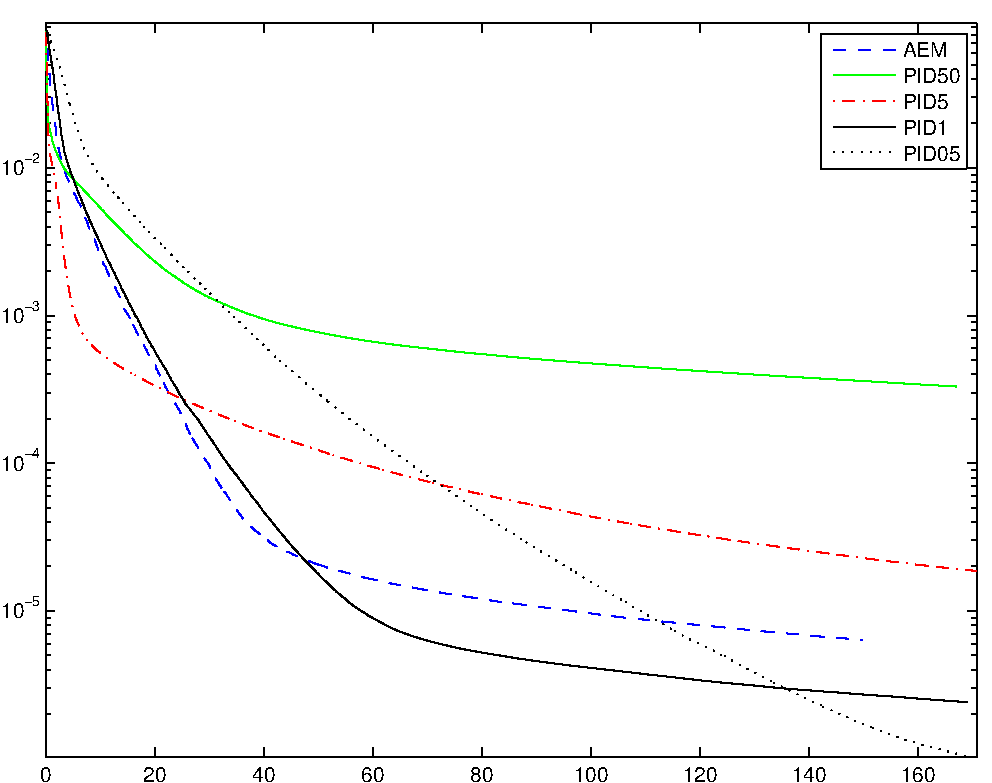
\includegraphics[width=10cm]{img/circles_err2}  \\
\mbox{LCR-1} \\
\\
\\
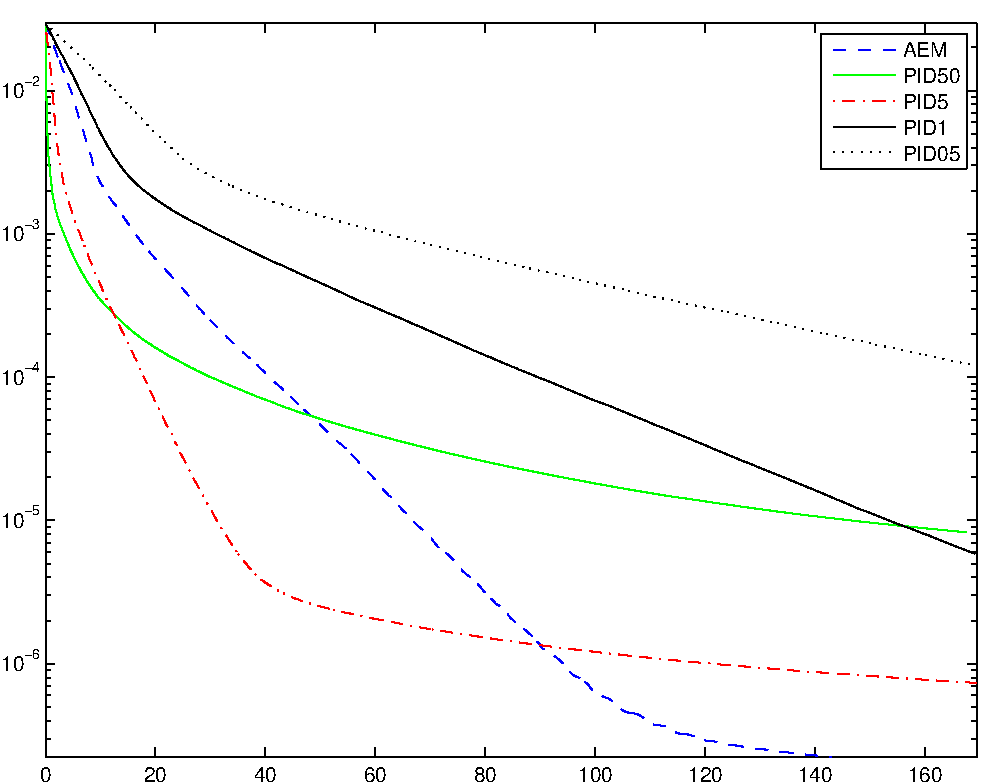
\includegraphics[width=10cm]{img/circles_10_err2} \\
\mbox{LCR-10} \\
\end{array}$
\end{center}
\end{figure}

\begin{figure}[H]
\begin{center}$
\begin{array}{cc}
\\
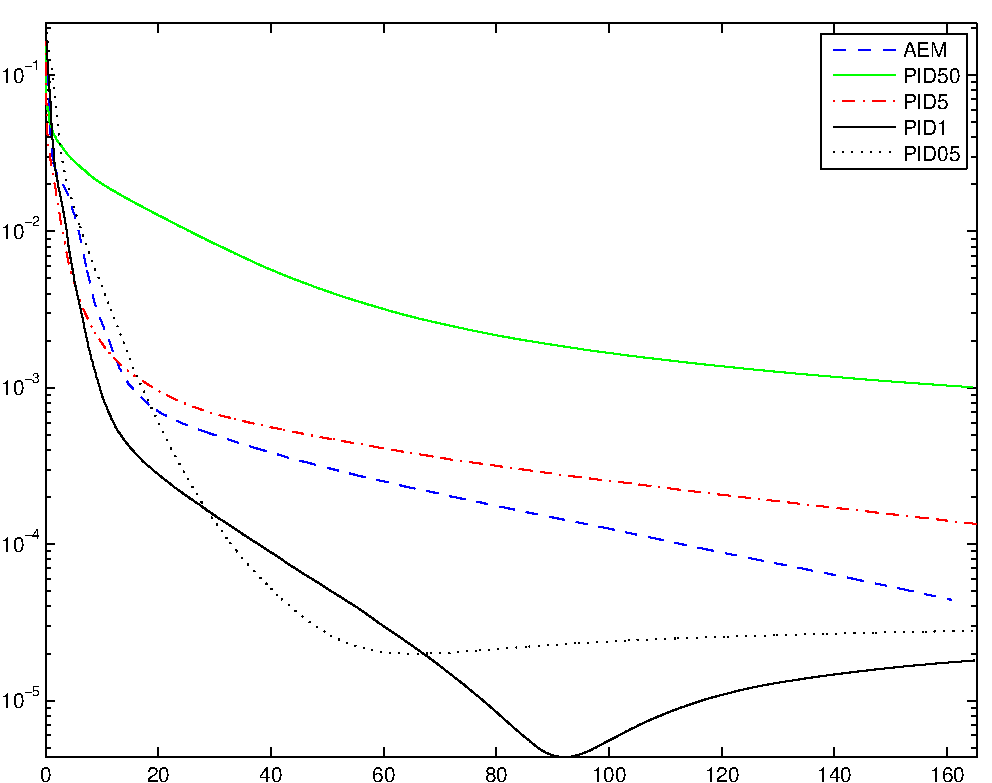
\includegraphics[width=10cm]{img/circles_d5_err2} \\
\mbox{LCR-0.2} \\
\\
\\
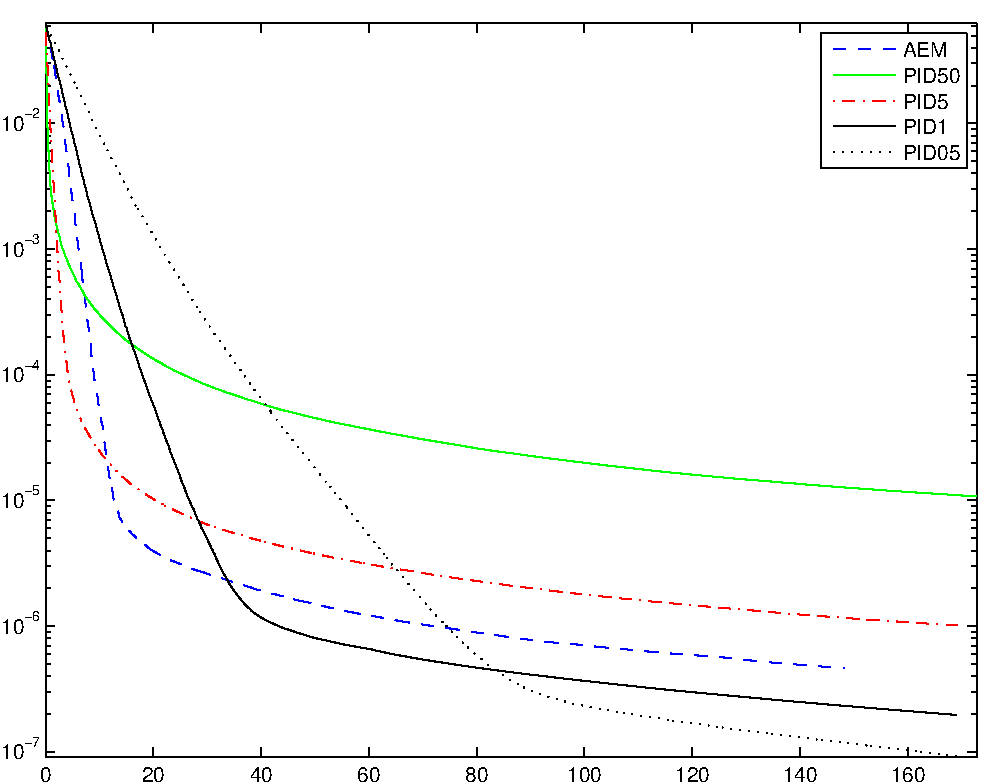
\includegraphics[width=10cm]{img/airplane_err2} \\
\mbox{Airplane} \\
\end{array}$
\end{center}
\end{figure}

\begin{figure}[H]
\begin{center}$
\begin{array}{c}
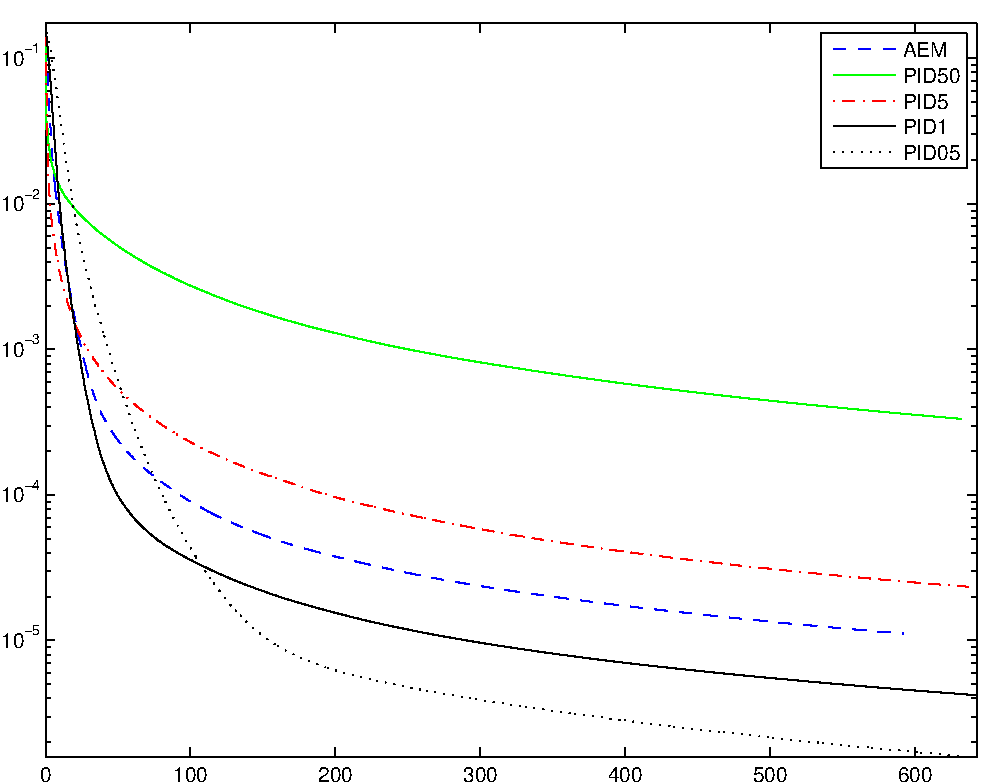
\includegraphics[width=10cm]{img/Panoramica_err2} \\
\mbox{DR} \\
\end{array}$
\end{center}
\end{figure}

%% inizio 5 sec

In order to evaluate the initial rate of convergence of the methods, we stopped both the algorithms after 5 seconds. In Table \ref{tab:5sec} we report the number of iterations performed and the corresponding reconstruction error $e$.


\begin{table}[H]
\begin{center}
\renewcommand*{\arraystretch}{1.5}
\begin{tabular}{|C{1.2cm}|C{0.9cm}|C{1.7cm}|C{0.9cm}|C{1.7cm}|C{0.9cm}|C{1.7cm}|}\hline
Method & \multicolumn{2}{c|} {LCR-1}  & \multicolumn{2}{c|} {LCR-10} & \multicolumn{2}{c|} {LCR-0.2} \\ \hline
     & \emph{iter} & $e^{(iter)}$ & \emph{iter}  & $e^{(iter)}$ & \emph{iter}  & $e^{(iter)}$ \\ \hline
AEM & 95 & 0.0236706 & 99 & 0.01113338 & 86 & 0.0444788 \\ \hline
PID50 & 90 & 0.0270578 & 91 & 0.00845165 & 98 & 0.0542035 \\ \hline
PID5 & 93 & 0.0250121 & 92 & 0.0078265 & 97 & 0.0453821 \\ \hline
PID1 & 92 & 0.0227458 & 92 & 0.0140898 & 91 & 0.0439414 \\ \hline
PID05 & 88 & 0.028708 & 93 & 0.020299 & 93 & 0.043499 \\ \hline
 & \multicolumn{2}{c|} {Airplane}  & \multicolumn{2}{c|}{DR} & \multicolumn{2}{c}{} \\ \cline{1-5}
     & \emph{iter} & $e^{(iter)}$ & \emph{iter}  & $e^{(iter)}$ & \multicolumn{2}{c}{} \\ \cline{1-5}
AEM & 109 &  0.0221838 & 27 & 0.0293069  & \multicolumn{2}{c}{} \\      \cline{1-5}
PID50 & 91 & 0.021386 & 27 & 0.0284085  & \multicolumn{2}{c}{} \\      \cline{1-5}
PID5 & 88 & 0.0213743 & 27 & 0.0286992  & \multicolumn{2}{c}{} \\      \cline{1-5}
PID1 & 91 & 0.024726 & 24 & 0.0472261  & \multicolumn{2}{c}{} \\      \cline{1-5}
PID05 & 91 & 0.0347613 & 24 & 0.0932484  & \multicolumn{2}{c}{} \\      \cline{1-5}
\end{tabular}
\caption{Number of iterations performed and reconstruction errors after 5 seconds.}
\label{tab:5sec}
\end{center}
\end{table}

In the following figures, we report the initial rate of convergence for both the algorithms, showing the relation between time and $e$ in the first 5 seconds.

\begin{figure}[H]
\begin{center}$
\begin{array}{c}
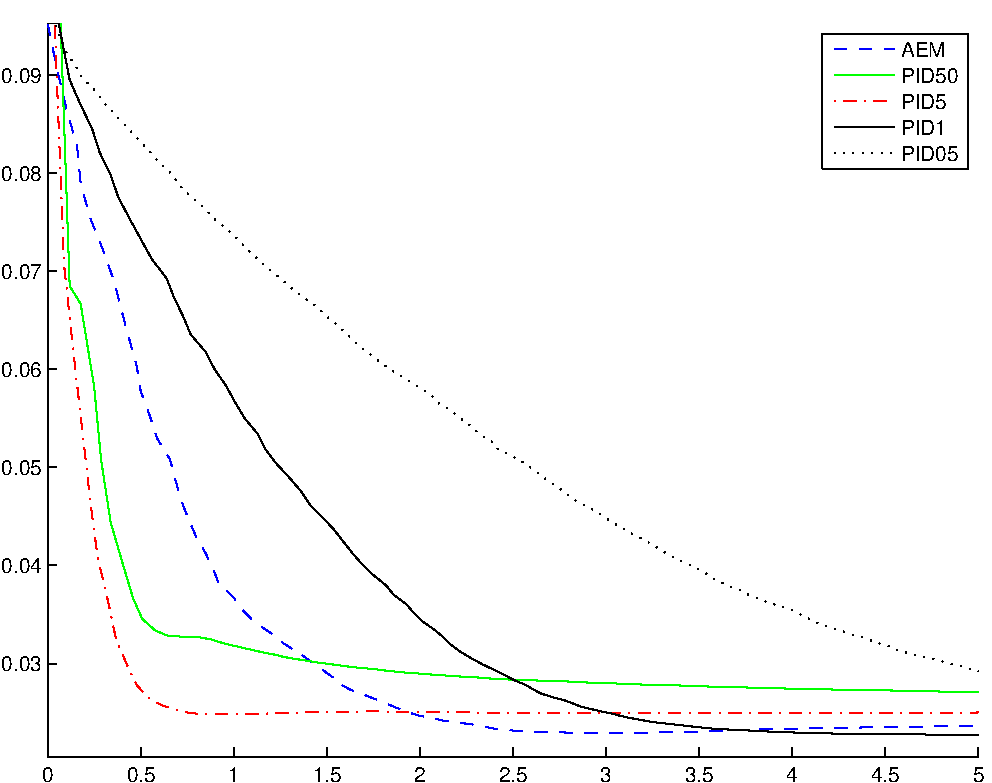
\includegraphics[width=10cm]{img/circles_err_5_sec}  \\
\mbox{LCR-1} \\
\\
\\
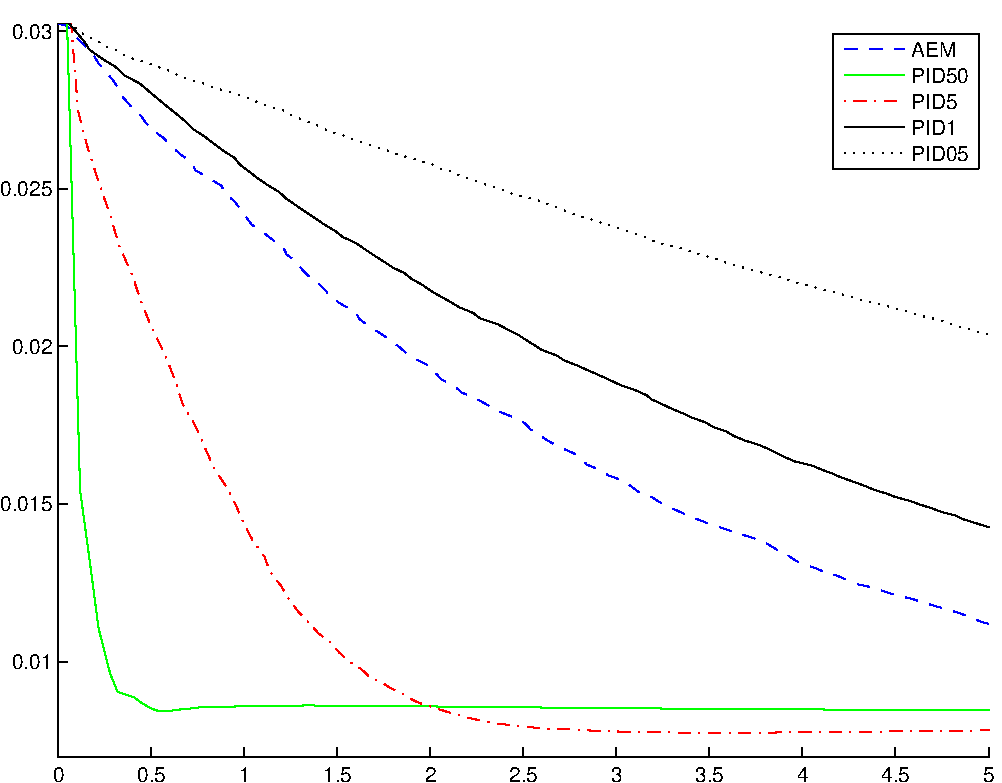
\includegraphics[width=10cm]{img/circles_10_err_5_sec} \\
\mbox{LCR-10} \\
\end{array}$
\end{center}
\caption{Behavior of relative reconstruction error in the first 5 seconds of the different methods for LCR-1 and LCR-10.}
\end{figure}

\begin{figure}[H]
\begin{center}$
\begin{array}{cc}
\\
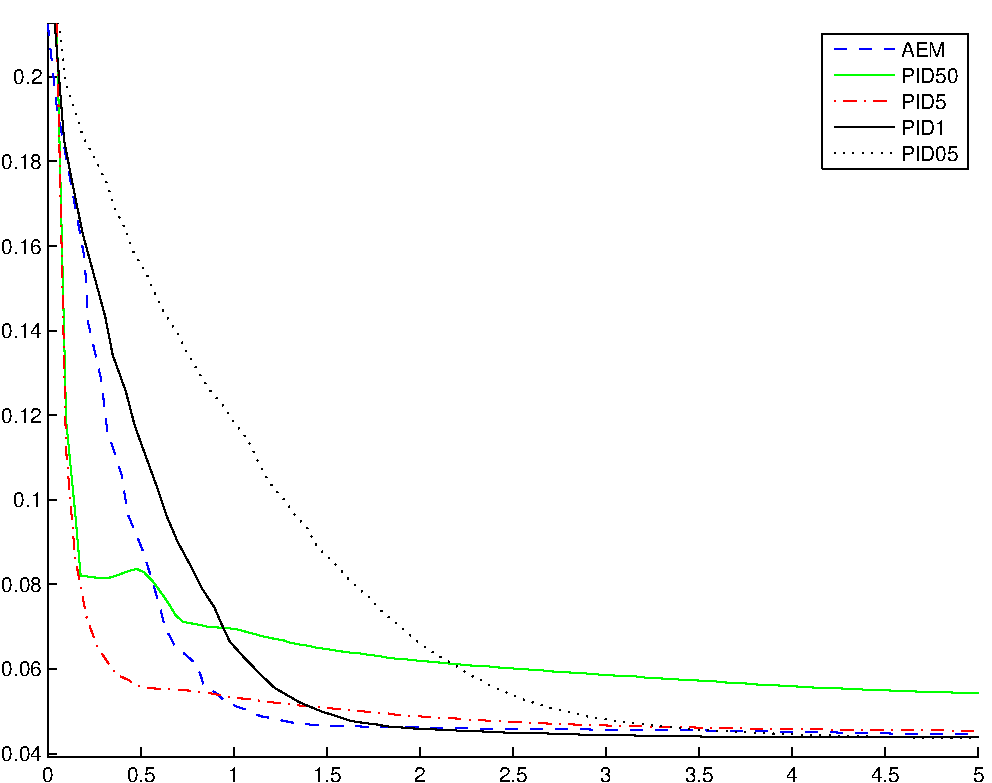
\includegraphics[width=10cm]{img/circles_d5_err_5_sec} \\
\mbox{LCR-0.2} \\
\\
\\
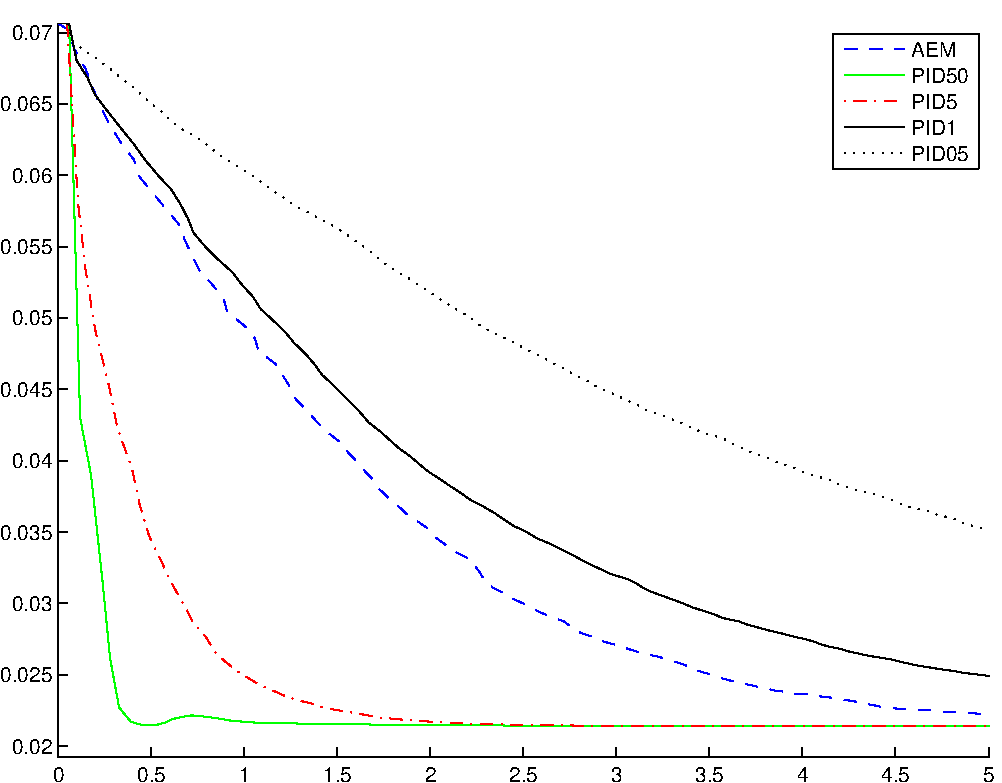
\includegraphics[width=10cm]{img/airplane_err_5_sec} \\
\mbox{Airplane} \\
\end{array}$
\end{center}
\caption{Behavior of relative reconstruction error in the first 5 seconds of the different methods for LCR-0.2 and Airplane.}
\end{figure}

\begin{figure}[H]
\begin{center}$
\begin{array}{c}
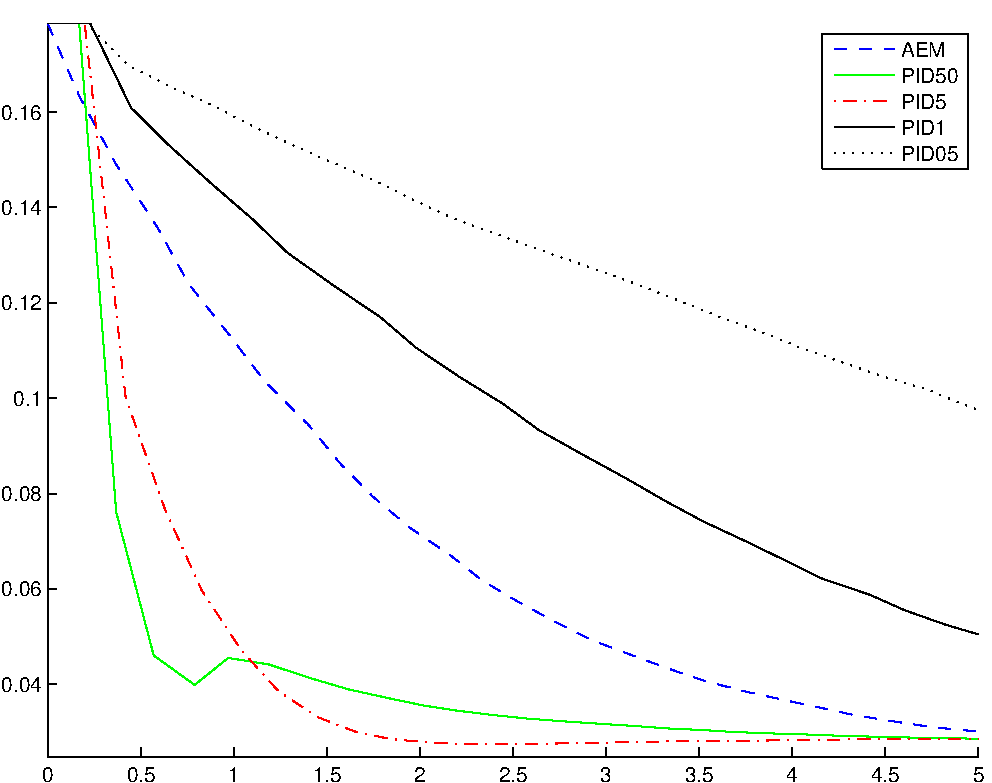
\includegraphics[width=10cm]{img/Panoramica_err_5_sec} \\
\mbox{DR} \\
\end{array}$
\end{center}
\caption{Behavior of relative reconstruction error in the first 5 seconds of the different methods for DR.}
\end{figure}

In order to evaluate if 5 seconds are enough to determine a good reconstruction of the image, we report the results after 5 seconds. For LCR-1, LCR-10, LCR-0.2, instead of the resulting image, we show the relation between the number of the column and the intensity, for the line 128.

\begin{figure}[H]
\begin{center}$
\begin{array}{cc}
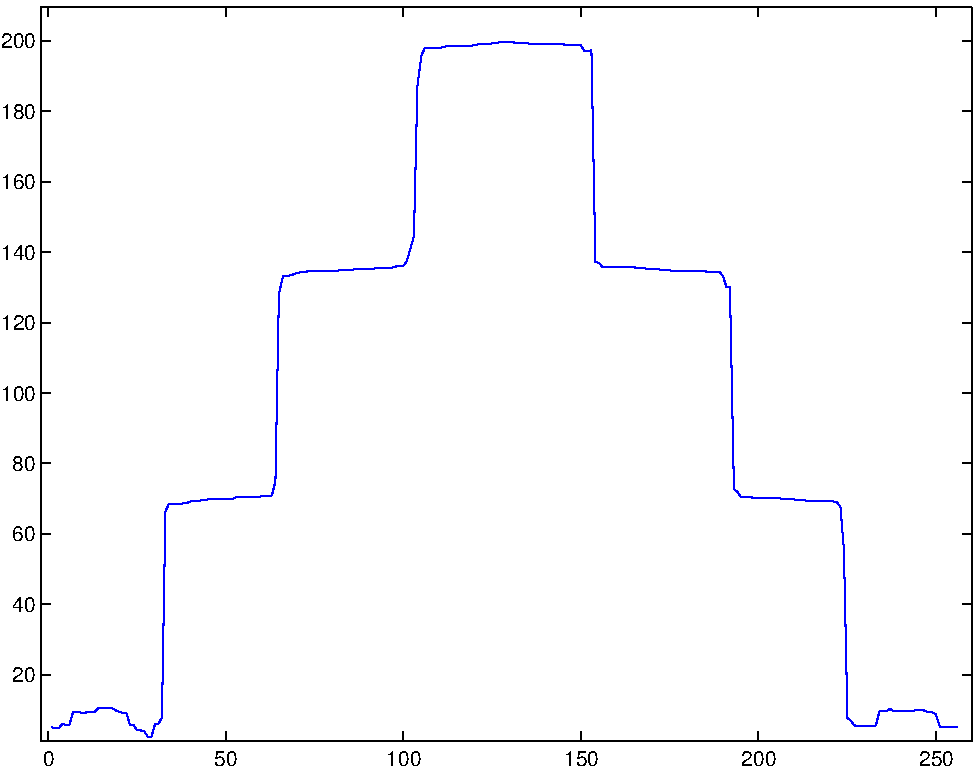
\includegraphics[width=6cm]{img/circles_it_95} & 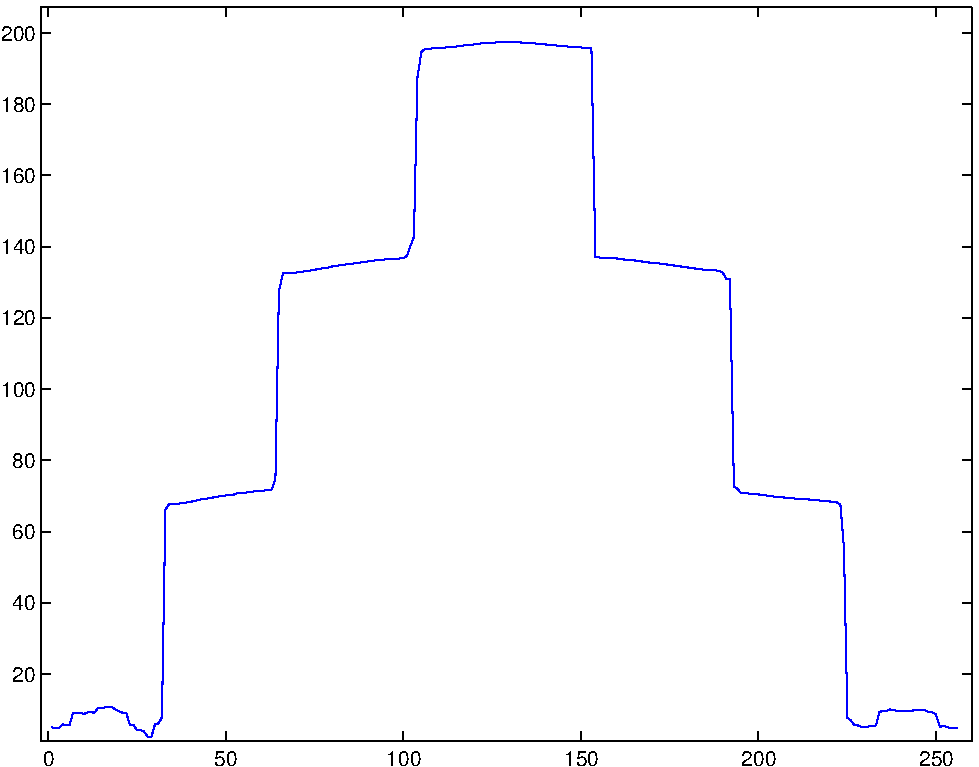
\includegraphics[width=6cm]{img/circles_PID_50_it_90} \\
\\
\mbox{AEM: 95 iterations} & \mbox{PID50: 90 iterations} \\
\\
\\
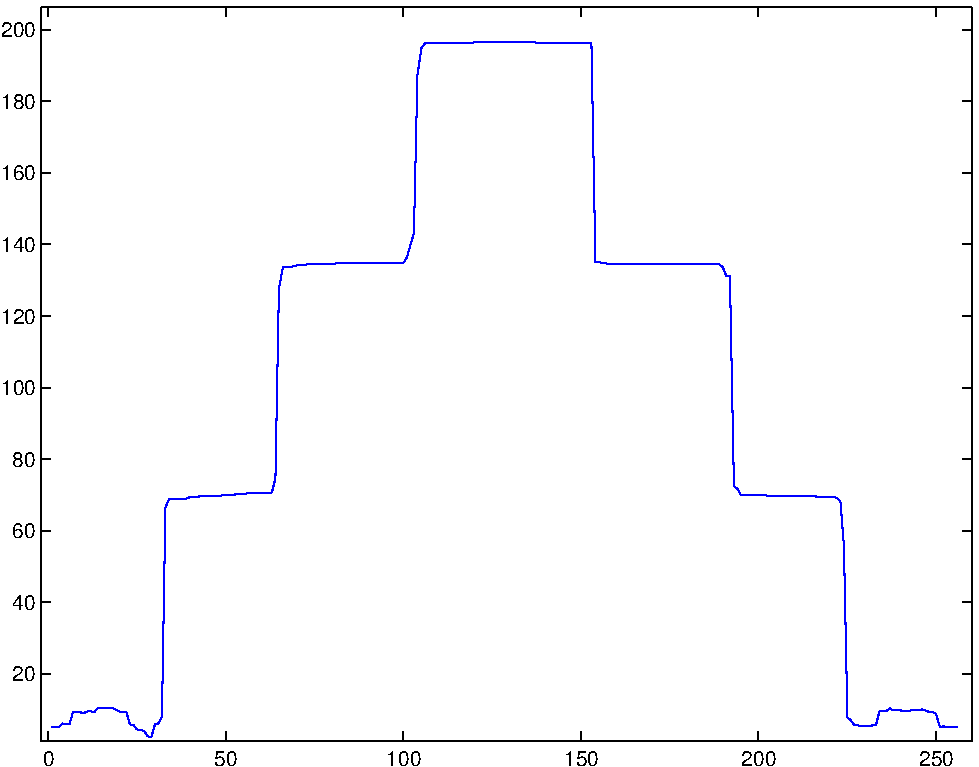
\includegraphics[width=6cm]{img/circles_PID_5_it_93} & 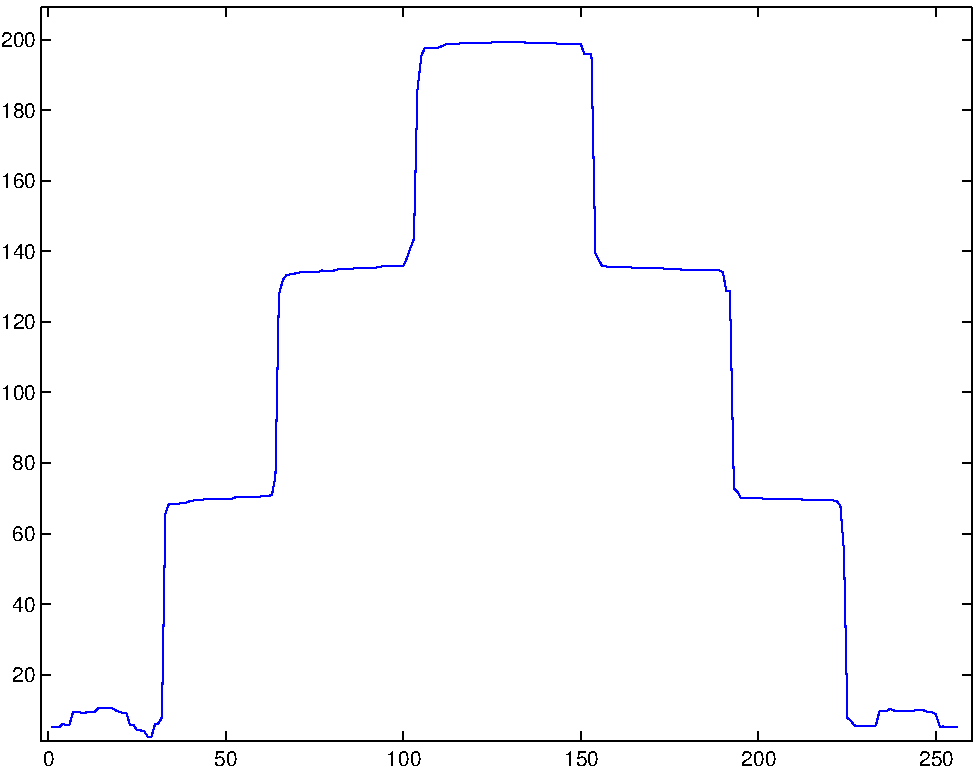
\includegraphics[width=6cm]{img/circles_PID_1_it_92} \\
\\
\mbox{PID5: 93 iterations} & \mbox{PID1: 92 iterations} \\
\\
\\
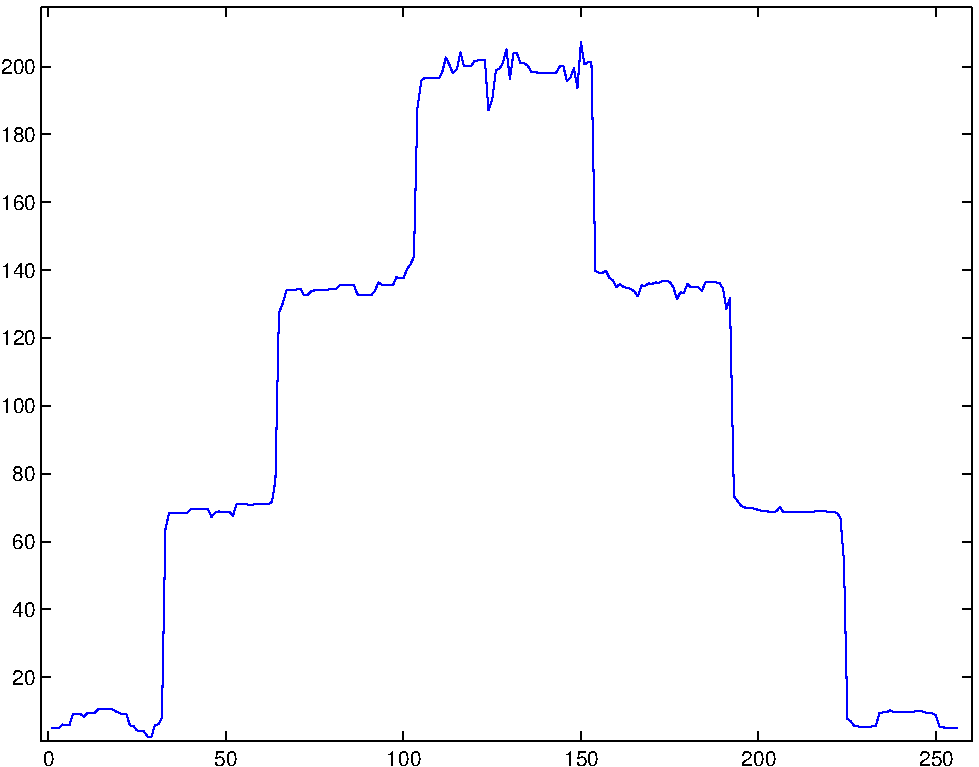
\includegraphics[width=6cm]{img/circles_PID_05_it_88} & \\
\\
\mbox{PID05: 88 iterations} &
\end{array}$
\end{center}
\caption{Line 128 of LCR-1 after 5 seconds}
\end{figure}

%%lcr-10

\begin{figure}[H]
\begin{center}$
\begin{array}{cc}
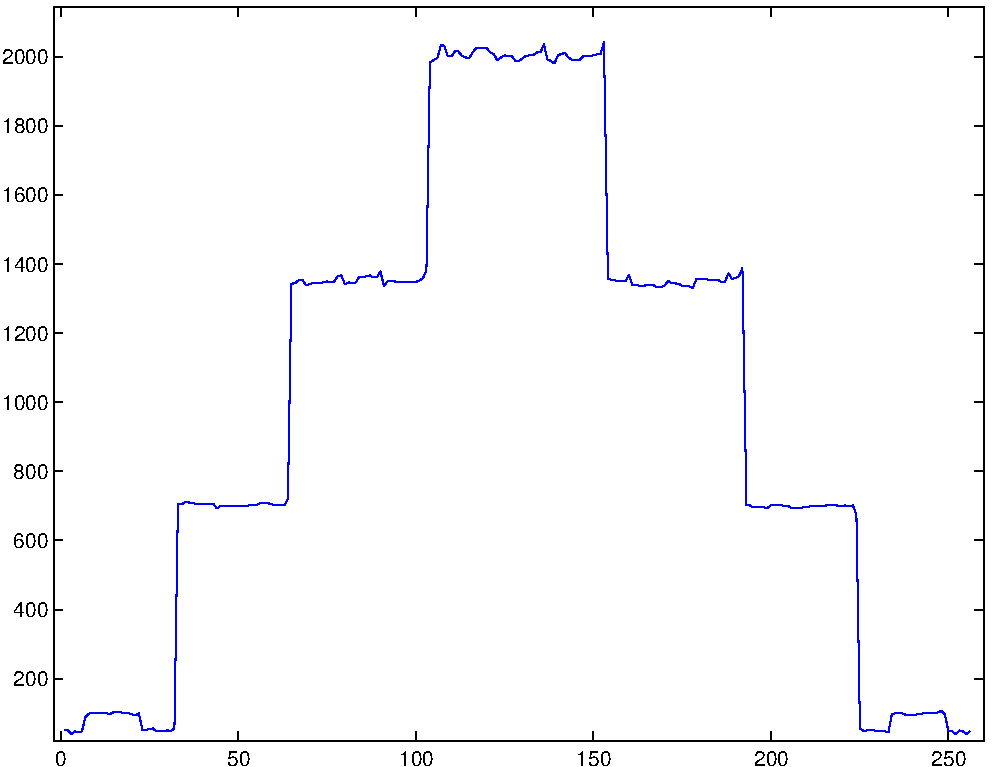
\includegraphics[width=6cm]{img/circles_10_it_99} & 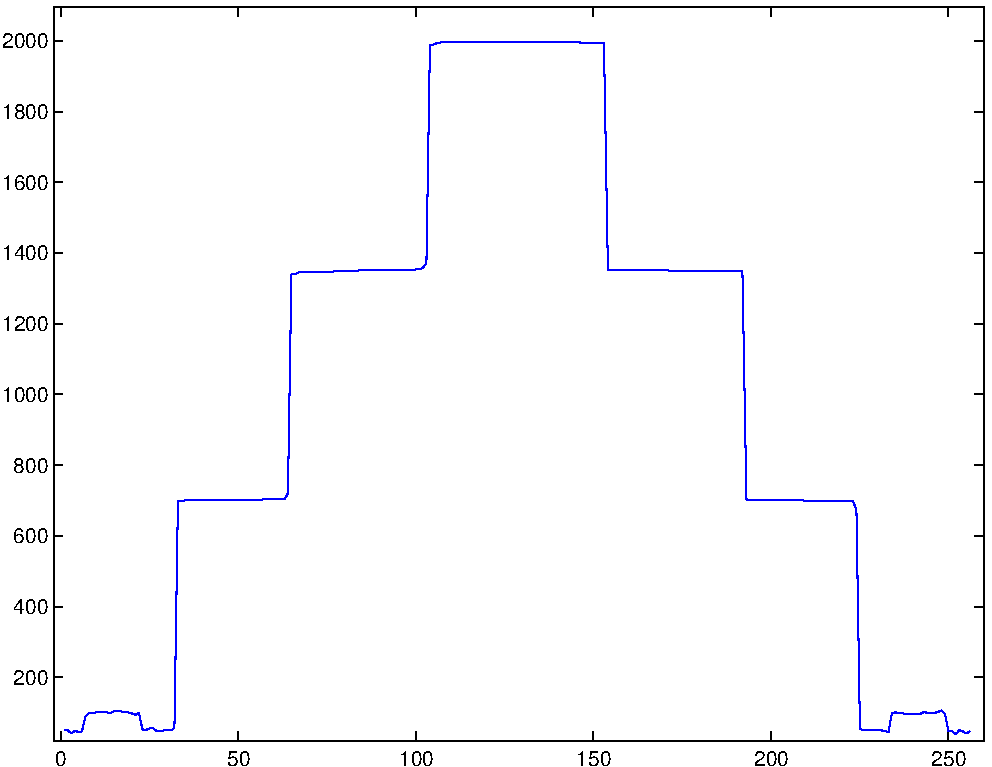
\includegraphics[width=6cm]{img/circles_10_PID_50_it_91} \\
\\
\mbox{AEM: 99 iterations} & \mbox{PID50: 91 iterations} \\
\\
\\
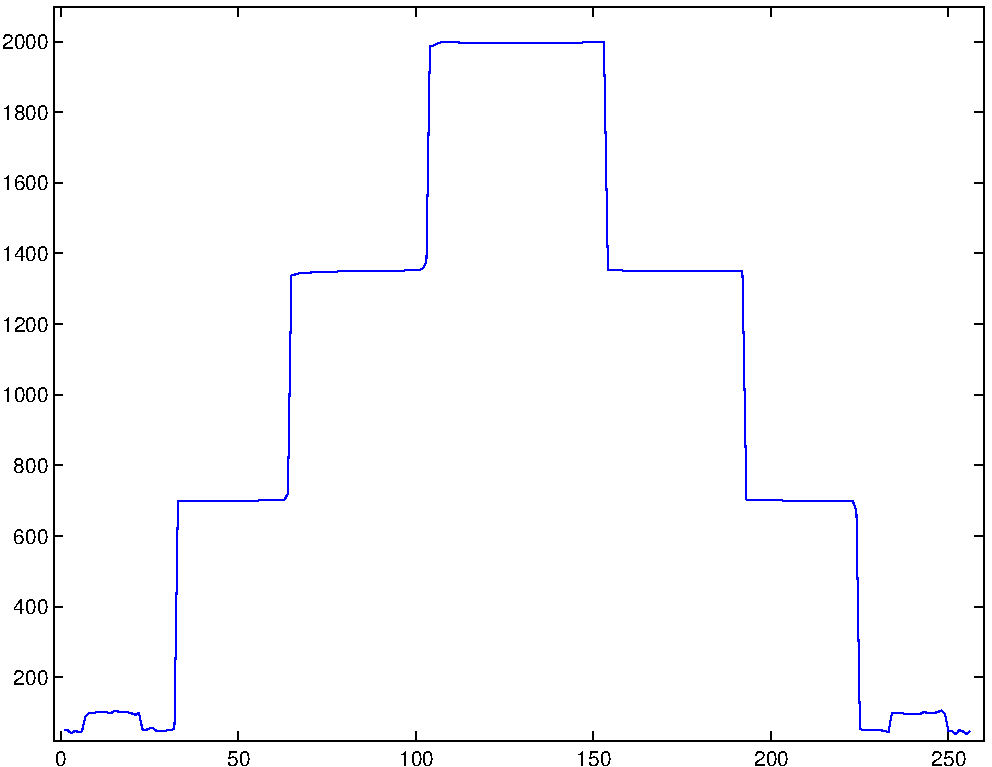
\includegraphics[width=6cm]{img/circles_10_PID_5_it_92} & 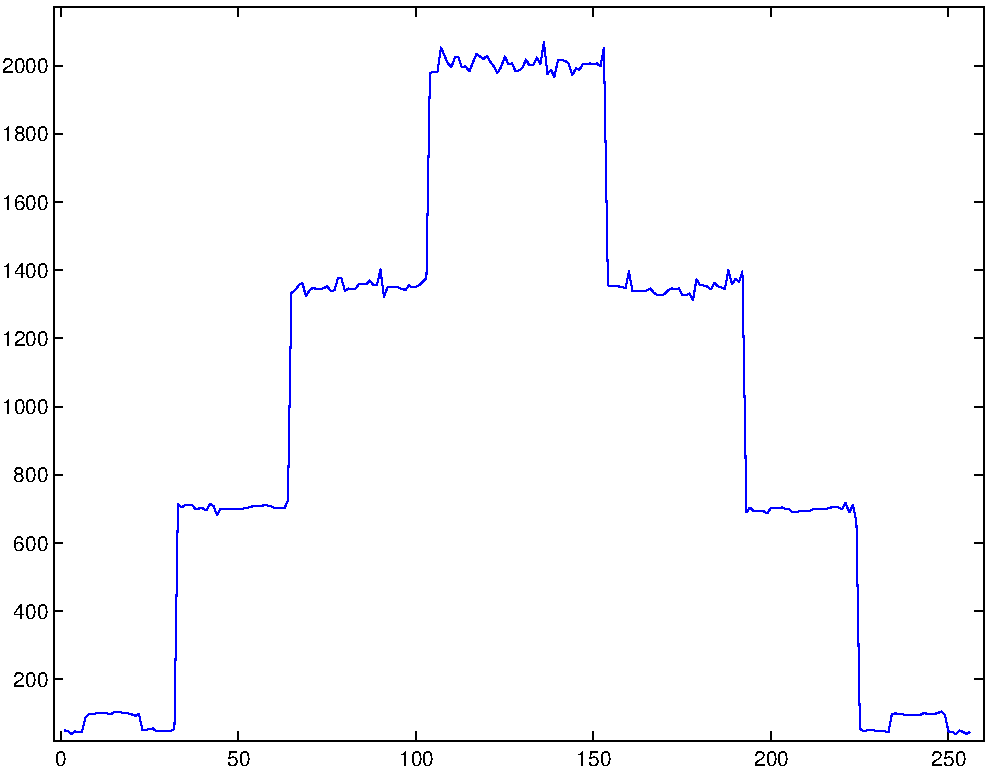
\includegraphics[width=6cm]{img/circles_10_PID_1_it_92} \\
\\
\mbox{PID5: 92 iterations} & \mbox{PID1: 92 iterations} \\
\\
\\
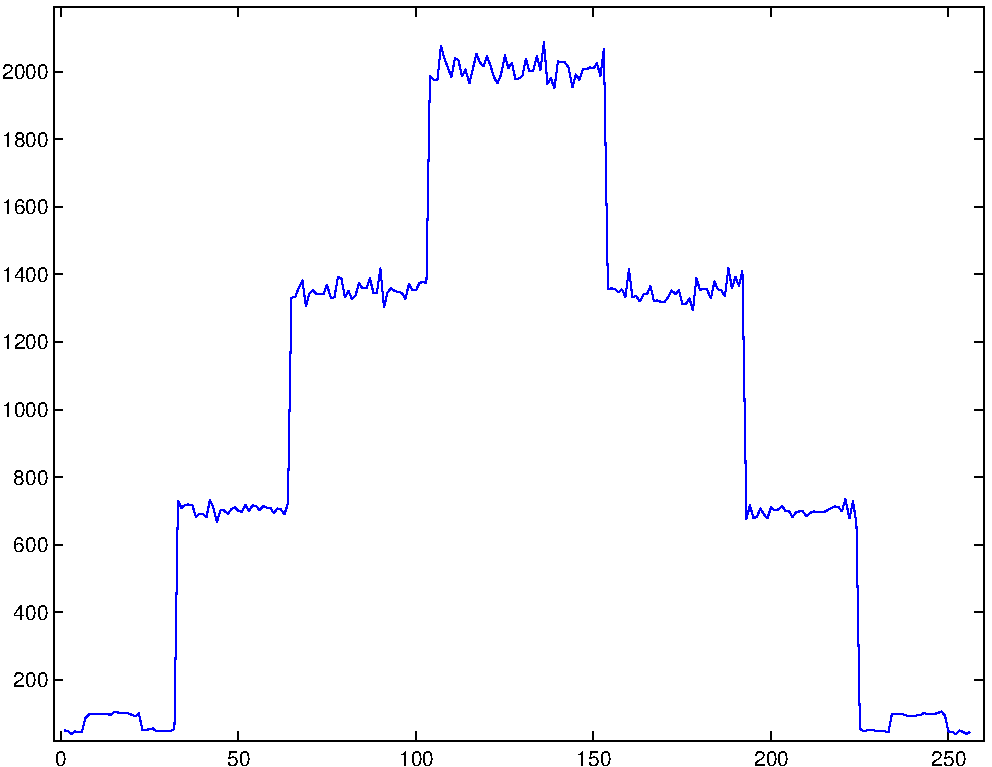
\includegraphics[width=6cm]{img/circles_10_PID_05_it_93} & \\
\\
\mbox{PID05: 93 iterations} &
\end{array}$
\end{center}
\caption{Line 128 of LCR-10 after 5 seconds}
\end{figure}

%% lcr-0.2

\begin{figure}[H]
\begin{center}$
\begin{array}{cc}
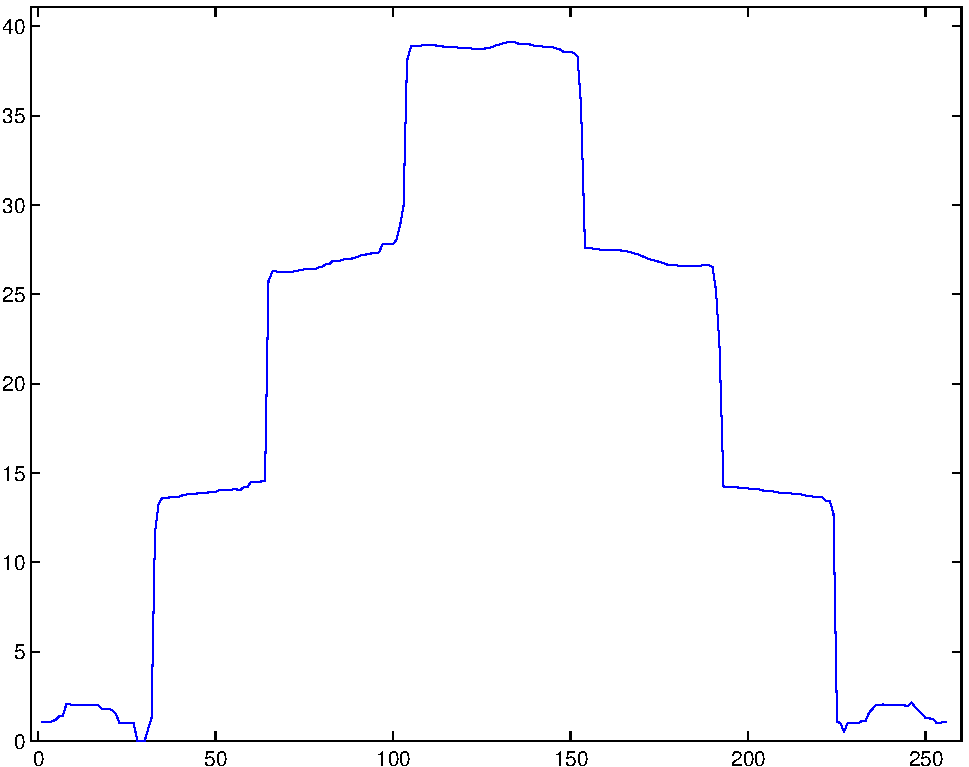
\includegraphics[width=6cm]{img/circles_d5_it_86} & 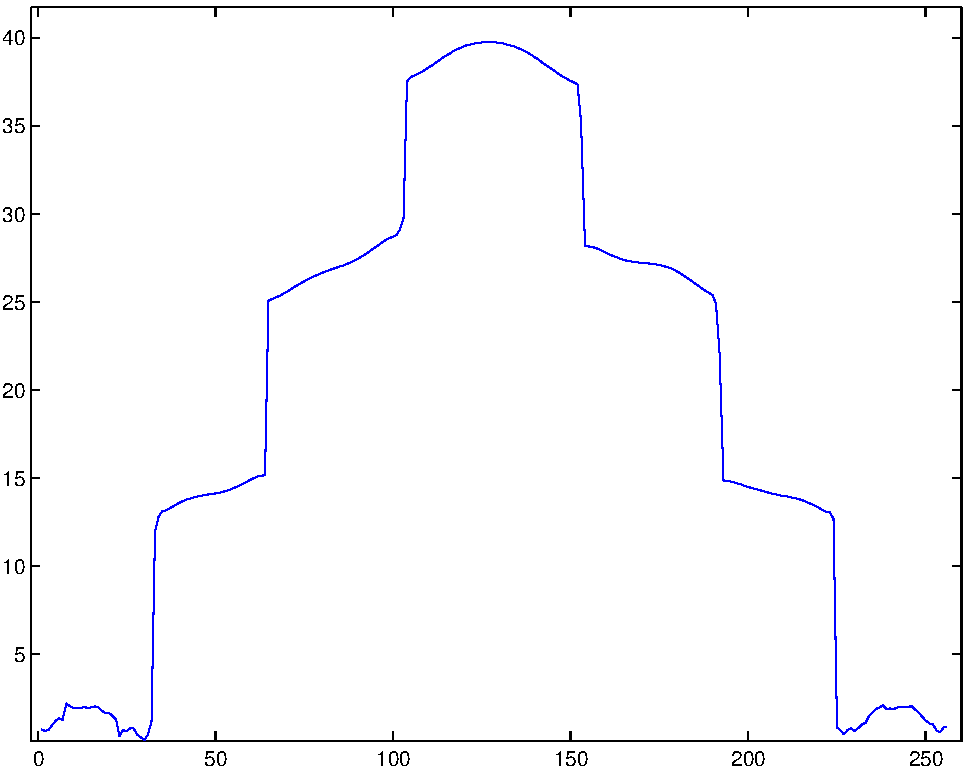
\includegraphics[width=6cm]{img/circles_d5_PID_50_it_98} \\
\\
\mbox{AEM: 86 iterations} & \mbox{PID50: 98 iterations} \\
\\
\\
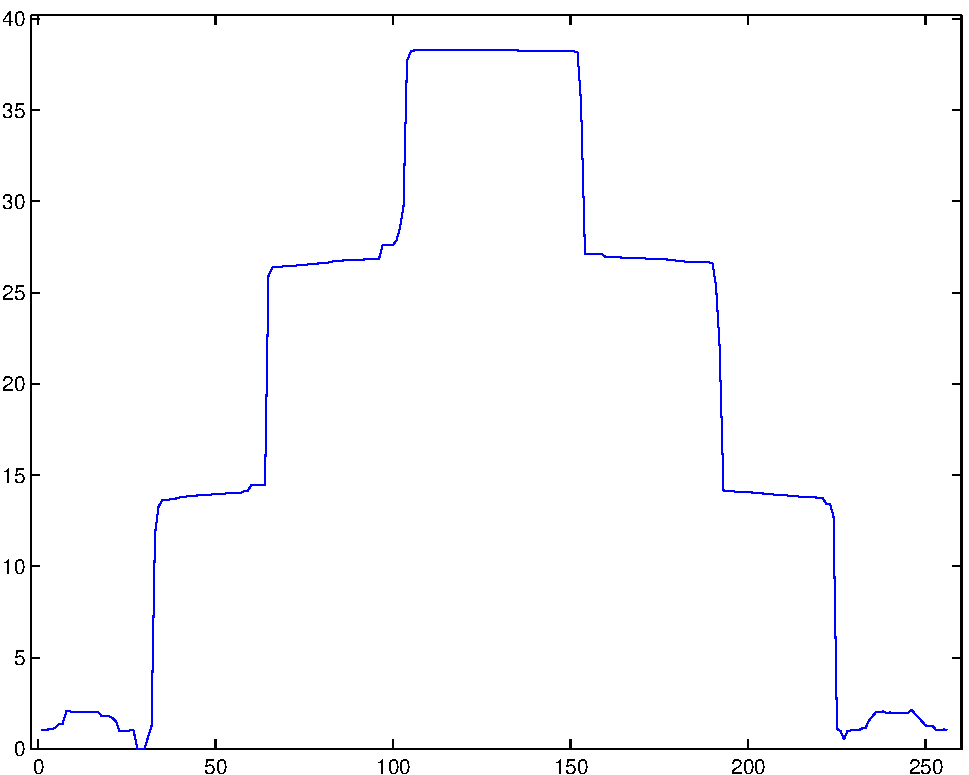
\includegraphics[width=6cm]{img/circles_d5_PID_5_it_97} & 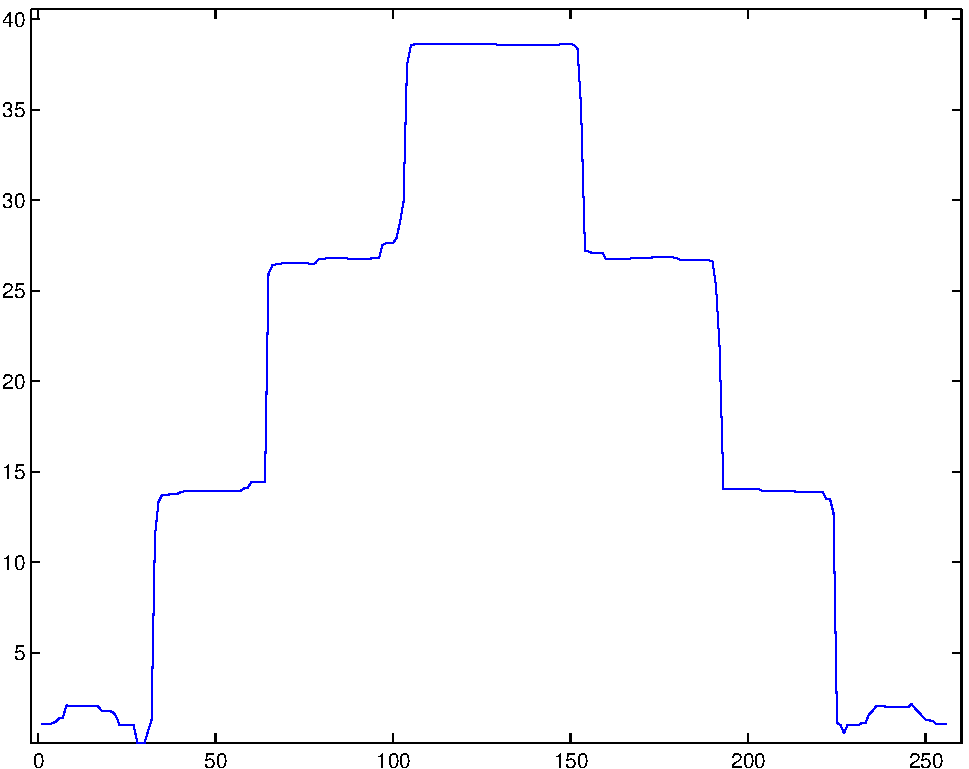
\includegraphics[width=6cm]{img/circles_d5_PID_1_it_91} \\
\\
\mbox{PID5: 97 iterations} & \mbox{PID1: 91 iterations} \\
\\
\\
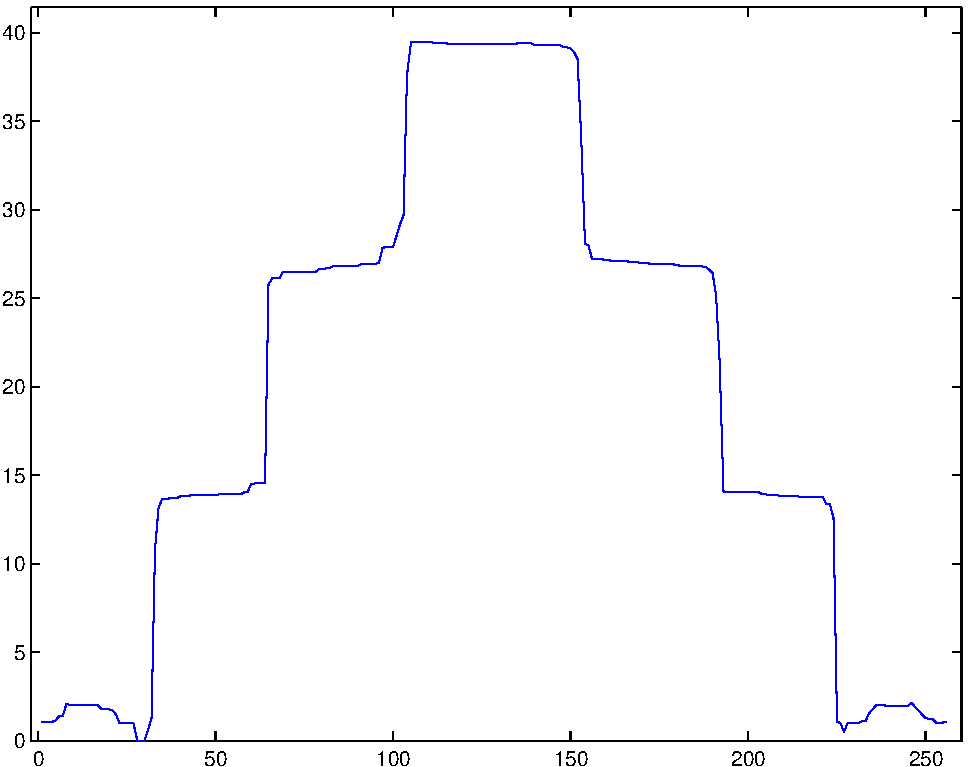
\includegraphics[width=6cm]{img/circles_d5_PID_05_it_93} & \\
\\
\mbox{PID05: 93 iterations} &
\end{array}$
\end{center}
\caption{Line 128 of LCR-0.2 after 5 seconds}
\end{figure}

%% airplane

\begin{figure}[H]
\begin{center}$
\begin{array}{cc}
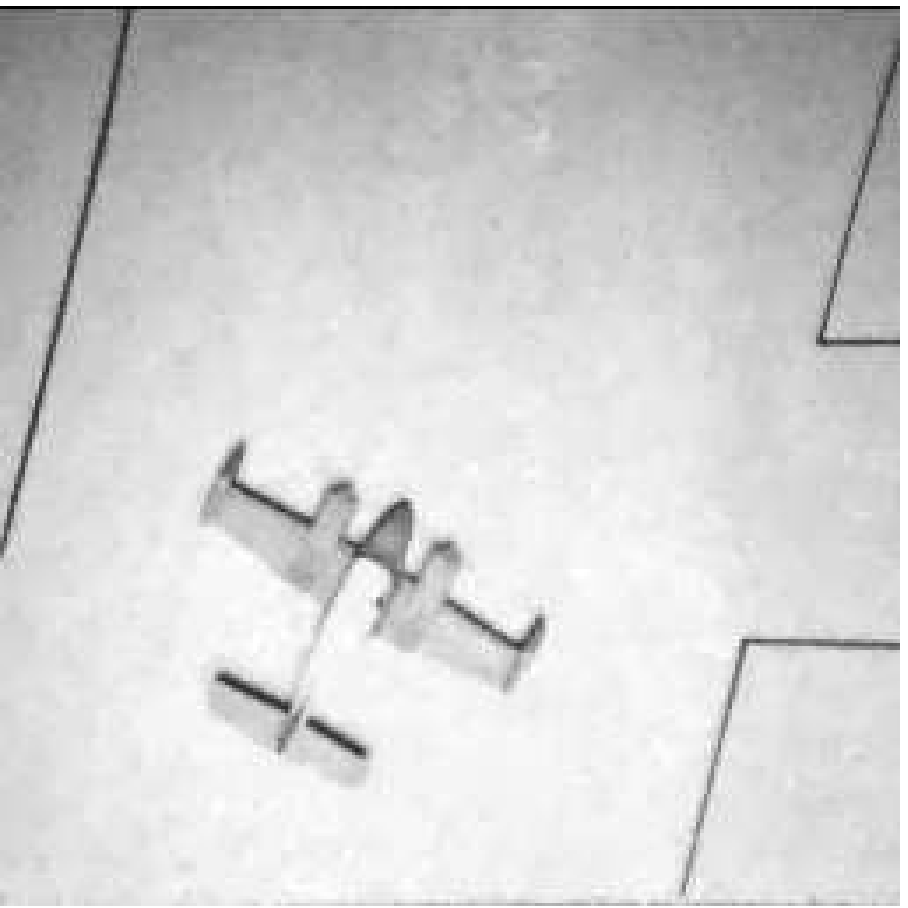
\includegraphics[width=4cm]{img/airplane_it_109} & 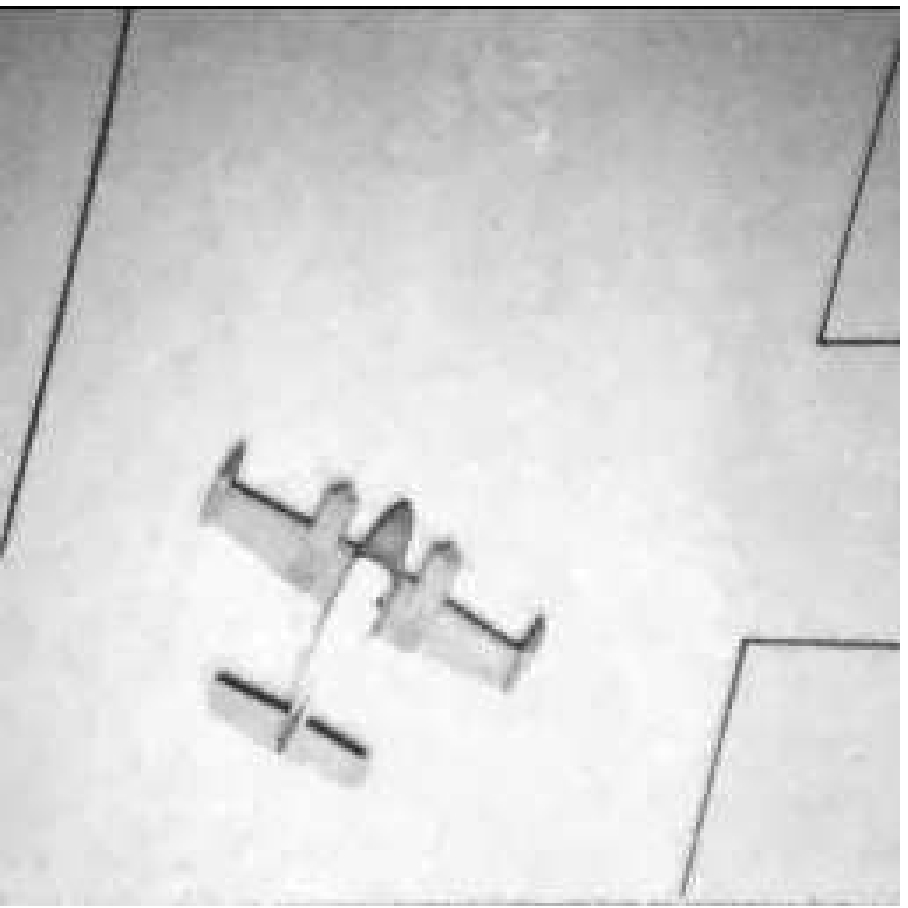
\includegraphics[width=4cm]{img/airplane_PID_50_it_91} \\
\\
\mbox{AEM: 109 iterations} & \mbox{PID50: 91 iterations} \\
\\
\\
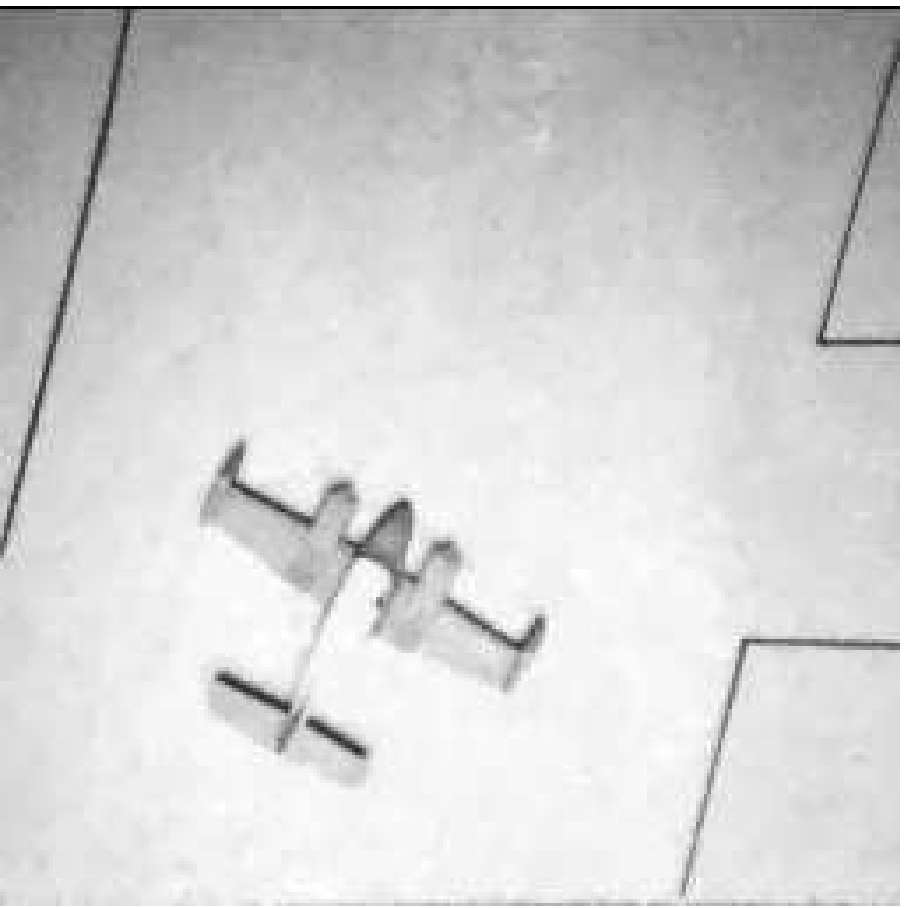
\includegraphics[width=4cm]{img/airplane_PID_5_it_88} & 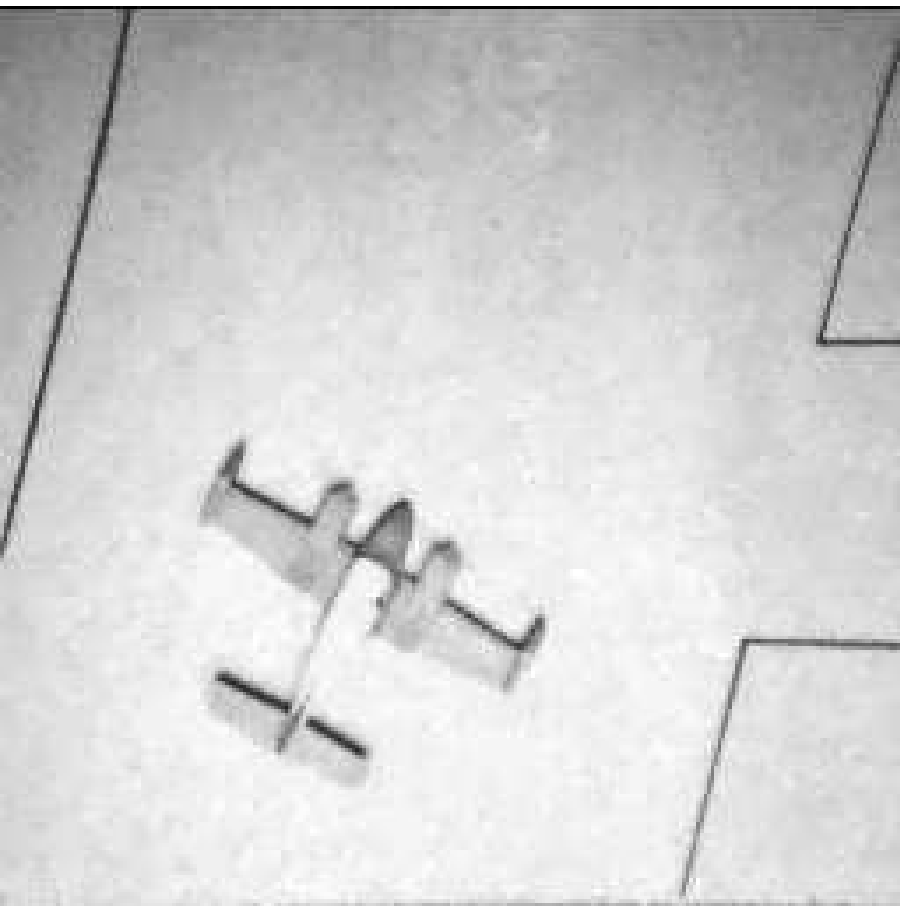
\includegraphics[width=4cm]{img/airplane_PID_1_it_91} \\
\\
\mbox{PID5: 88 iterations} & \mbox{PID1: 91 iterations} \\
\\
\\
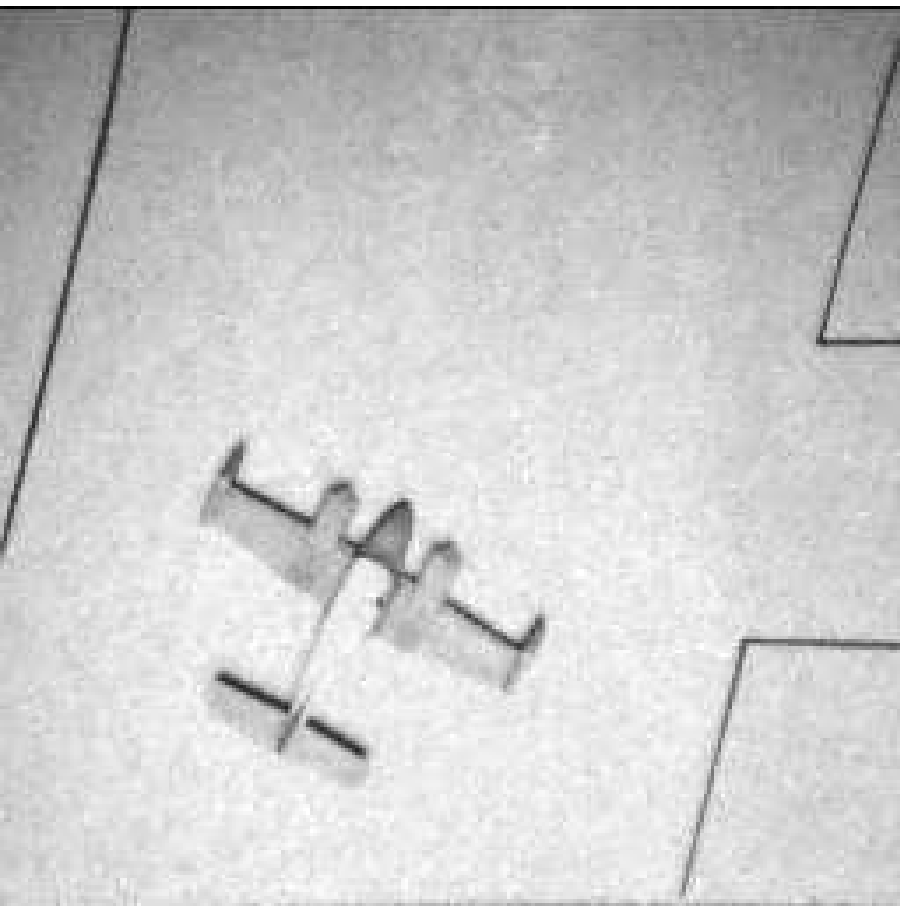
\includegraphics[width=4cm]{img/airplane_PID_05_it_91} & \\
\\
\mbox{PID05: 91 iterations} &
\end{array}$
\end{center}
\caption{Airplane after 5 seconds}
\end{figure}

%% panoramica

\begin{figure}[H]
\begin{center}$
\begin{array}{cc}
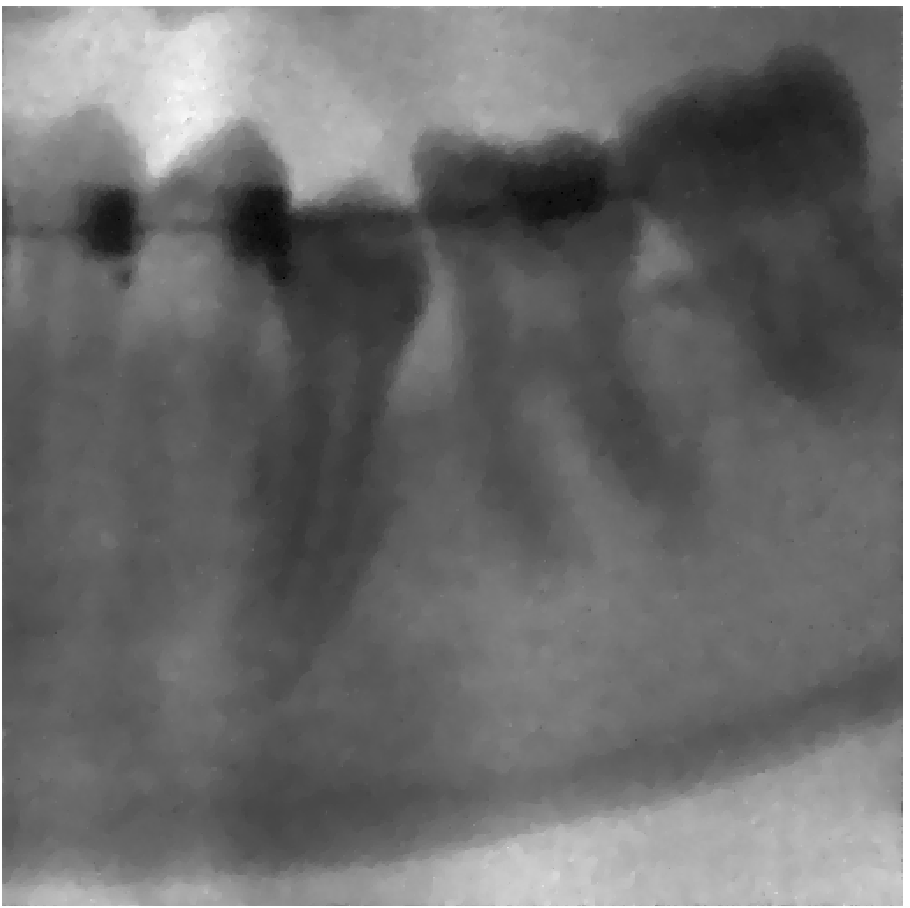
\includegraphics[width=6cm]{img/Panoramica_it_27} & 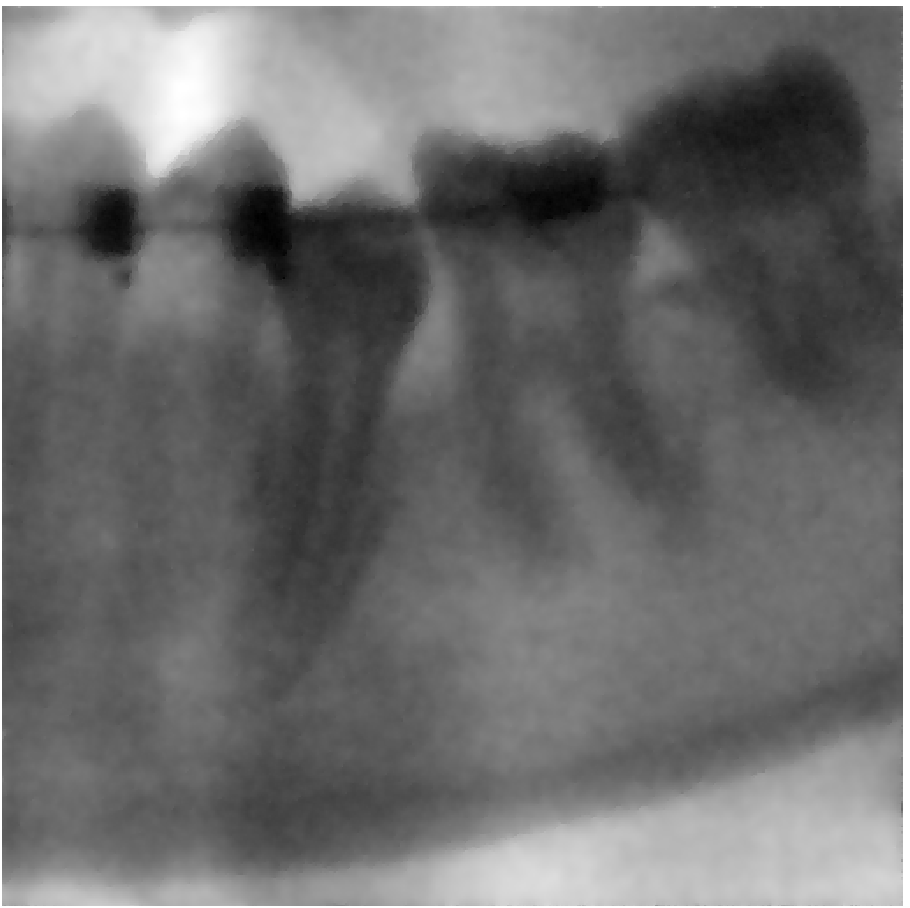
\includegraphics[width=6cm]{img/Panoramica_PID_50_it_27} \\
\mbox{AEM: 27 iterations} & \mbox{PID50: 27 iterations} \\
\\
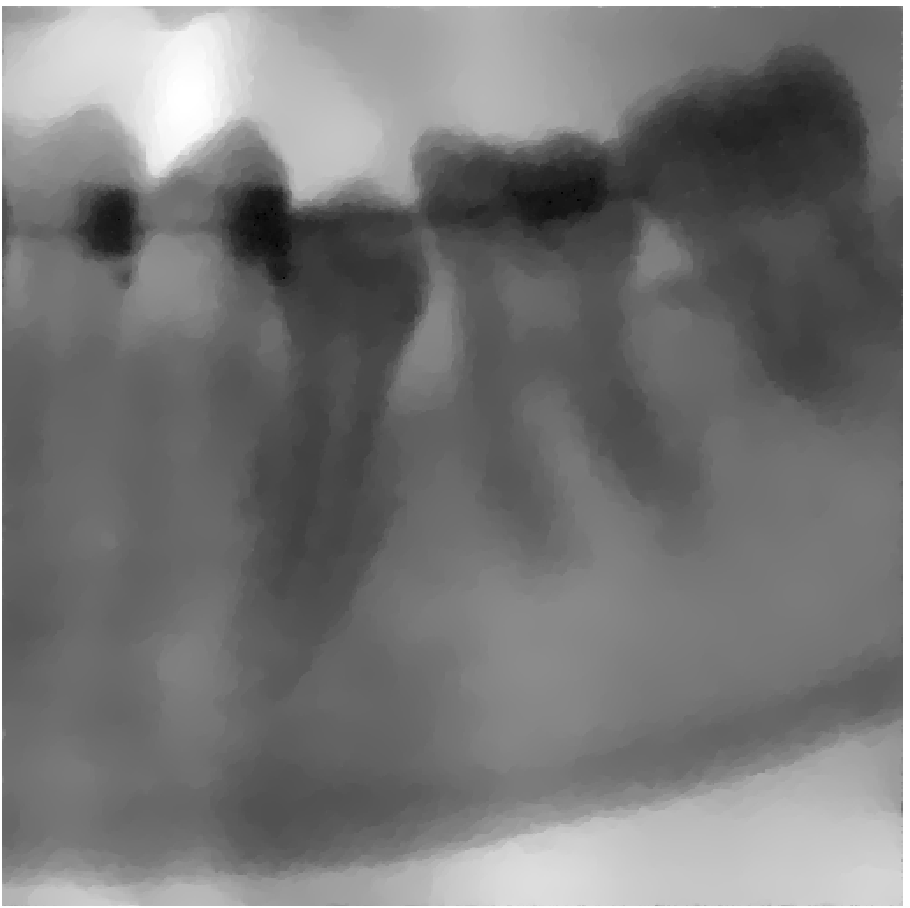
\includegraphics[width=6cm]{img/Panoramica_PID_5_it_27} & \includegraphics[width=6cm]{img/Panoramica_PID_1_it_24} \\
\mbox{PID5: 27 iterations} & \mbox{PID1: 24 iterations} \\
\\
\includegraphics[width=6cm]{img/Panoramica_PID_05_it_24} & \\
\mbox{PID05: 24 iterations} &
\end{array}$
\end{center}
\caption{DR after 5 seconds}
\end{figure}

From these results we can draw the following remarks.

\begin{itemize}
\item The rate of convergence of PIDSplit+ as a minimization method is strongly conditioned by the choice of the parameter $\gamma$: values which have been observed to give a good initial rate of convergence $\bigl($i.e. high values such as $\frac{50}{\beta}$ and $\frac{5}{\beta}\bigr)$ are not asymptotically satisfactory and \emph{vice versa}.

\item In terms of rates of convergence, AEM is instead located somewhat between the 4 different versions of PIDSplit+, regarding both the initial behavior and the asymptotic one.

\item Any iteration of AEM is, in general, less demanding in terms of computational complexity than any of PIDSplit+, since in the latter the solution of a system is required at each step with the Fast Fourier Transform algorithm (see section \ref{app:circ}).

\item AEM is self-consistent, since it does not depend from any parameter, because the choice of the steplength is adaptive; however, an optimal choice of the parameter $\gamma$ for the PIDSplit+ may provide good results even faster than AEM.

\item If the image considered has a high signal-to-noise ratio (as LCR-0.2) or is significantly bigger than the others (as DR), AEM is observed to have an overall good behavior with respect to the reconstruction error $e^{(rec)}$ also at the initial steps.

\end{itemize}

\section{Behavior of AEM and PIDSplit+ with real-world problems}

In the second set of experiments, considering the images from the project ``PRISMA'', we first compute the optimal value $\beta_{disc}$ for $\beta$, using the discrepancy principle \eqref{discr} proposed in \citep{discr_princ}.

In order to solve the nonlinear equation in $\beta$ involved in the principle, we use a bisection method with the tolerance of $10^{-3}$ combined with AEM to evaluate $x_{\beta}^*$, with the maximum number of iterations set at 3000. The results are the following:

\begin{table}[H]
\begin{center}
\renewcommand*{\arraystretch}{1.6}
\begin{tabular}{|C{1.8cm}|C{2.2cm}|}
\hline
Problem & $\beta_{disc}$ \\
\hline
Image11 & 0.3119 \\ \hline
Image13 & 0.317748 \\ \hline
Image22 & 0.31385 \\ \hline
Image48 & 0.31385 \\ \hline
Image49 & 0.309951 \\ \hline
Image50 & 0.31385 \\
\hline
\end{tabular}
\caption{Values of $\beta_{disc}$ for each image.}
\end{center}
\end{table}

In order to understand the efficacy of such discrepancy principle, we examine some values in the left neighborhood of $\beta_{disc}$, defining as $\beta_{opt}$ the one which provides, among them, the lowest reconstruction error with respect to the ground truth image. Such relative reconstruction error is defined, as previously, as:

$$e^{(iter)} =  \dfrac{||x^{(iter)}-x^*||_2}{||x^*||_2}$$

where $x^*$ is now the ground truth.

The results are shown in the following tables (the line in bold represents the value of $\beta$ chosen as $\beta_{opt}$):

\begin{table}[H]
\begin{center}
\renewcommand*{\arraystretch}{1.6}
\begin{tabular}{|C{1.8cm}|C{1cm}|C{2.2cm}|C{2.2cm}|C{2.2cm}|}
\hline
Problem & $\beta$ & $e^{(3000)}$ & KL & TV \\ \hline
 & 0.01 & 0.0177422 & 2149.67 & 940135 \\ \cline{2-5}
 & \textbf{0.02} & \textbf{0.016393} & \textbf{3915.19} & \textbf{814481} \\ \cline{2-5}
 & 0.05 & 0.0164795 & 7272 & 709033 \\ \cline{2-5}
Image11 & 0.07 & 0.0175498 & 9217.41 & 676261 \\ \cline{2-5}
 & 0.1 & 0.0196065 &  12111.6 & 641869 \\ \cline{2-5}
 & 0.2 & 0.0272481 & 22348.4 & 571412\\ \cline{2-5}
 & 0.3 & 0.0348308 & 34156.3 & 523622\\
\hline
Problem & $\beta$ & $e^{(3000)}$ & KL & TV \\ \hline
 & 0.01 & 0.016544 & 2160.85 & 928899\\ \cline{2-5}
 & \textbf{0.02} & \textbf{0.0152543} & \textbf{3911.13} & \textbf{804136} \\ \cline{2-5}
 & 0.05 & 0.0157587 & 7220.98 & 700156\\ \cline{2-5}
Image13 & 0.07 & 0.0170977 & 9135.89 & 667931\\ \cline{2-5}
 & 0.1 & 0.0194859 & 11991.5 & 633970\\ \cline{2-5}
 & 0.2 & 0.027614 & 21957.3 & 565456\\ \cline{2-5}
 & 0.3 & 0.0353886 & 33566.1 & 518485\\
\hline
Problem & $\beta$ & $e^{(3000)}$ & KL & TV \\ \hline
 & 0.01 & 0.0162132 & 2198.92 & 941487\\ \cline{2-5}
 & \textbf{0.02} & \textbf{0.0148022} & \textbf{4025.25} & \textbf{811476} \\ \cline{2-5}
 & 0.05 & 0.0152197  & 7450.87 & 703634\\ \cline{2-5}
Image22 & 0.07 & 0.0165708 & 9409.18 & 670663\\ \cline{2-5}
 & 0.1 & 0.0190068 & 12318.1 & 636078\\ \cline{2-5}
 & 0.2 & 0.0272591 & 22447.1 & 566297\\ \cline{2-5}
 & 0.3 & 0.0350216 & 34060.9 & 519290\\ \cline{2-5}
\hline
\end{tabular}
\end{center}
\end{table}

\begin{table}[H]
\begin{center}
\renewcommand*{\arraystretch}{1.6}
\begin{tabular}{|C{1.8cm}|C{1cm}|C{2.2cm}|C{2.2cm}|C{2.2cm}|}
\hline
Problem & $\beta$ & $e^{(3000)}$ & KL & TV \\ \hline
 & 0.01 & 0.0154639 & 2157.87 & 932984\\ \cline{2-5}
 & \textbf{0.02} & \textbf{0.0139999} & \textbf{3917.88} & \textbf{807767} \\ \cline{2-5}
 & 0.05 & 0.0144383 & 7249.03 & 703296\\ \cline{2-5}
Image48 & 0.07 & 0.0157969 & 9165.57 & 671017\\ \cline{2-5}
 & 0.1 & 0.0182356 & 12013.4 & 637173\\ \cline{2-5}
 & 0.2 & 0.0267319 & 22221.7 & 566942\\ \cline{2-5}
 & 0.3 & 0.0346593 & 33915.8 & 519601\\
\hline
Problem & $\beta$ & $e^{(3000)}$ & KL & TV \\ \hline
 & 0.01 & 0.0160722 & 2159.3 & 940036\\ \cline{2-5}
 & \textbf{0.02} & \textbf{0.0145997} & \textbf{3949.21} & \textbf{812753} \\ \cline{2-5}
 & 0.05 & 0.148771 & 7346.71 & 706008\\ \cline{2-5}
Image49 & 0.07 & 0.0161719 & 9307.99 & 672987\\ \cline{2-5}
 & 0.1 & 0.0185724 & 12237.8 & 638159\\ \cline{2-5}
 & 0.2 & 0.0268924 & 22499.1 & 567536\\ \cline{2-5}
 & 0.3 & 0.0348179 & 34338.2 & 519626\\
\hline
Problem & $\beta$ & $e^{(3000)}$ & KL & TV \\ \hline
 & 0.01 & 0.0158575 & 2175.75 & 932012\\ \cline{2-5}
 & \textbf{0.02} & \textbf{0.0144898} & \textbf{3963.06} & \textbf{804892} \\ \cline{2-5}
 & 0.05 & 0.0150870 & 7921.30 & 699159\\ \cline{2-5}
Image50 & 0.07 & 0.0165020 & 9225.63 & 667082\\ \cline{2-5}
 & 0.1 & 0.0902397 & 12087.30 & 633079\\ \cline{2-5}
 & 0.2 & 0.0276045 & 22290.52 & 562893\\ \cline{2-5}
 & 0.3 & 0.0355275 & 33892.61 & 515937\\
\hline
\end{tabular}
\end{center}
\end{table}


Using both $\beta_{opt}$ and $\beta_{disc}$ we run AEM and PIDSplit+ for all of the images considered, setting a maximum number of 3000 iterations and using the following stopping criterion:

\begin{align}
\label{stopping}
\dfrac{||w^{(k+1)}-w^{(k)}||_2}{||w^{(k+1)}||_2} < 10^{-6}
\end{align}

where, for AEM:

$$w^{(k)} = \left( x^{(k)} , y^{(k)} \right)^T$$

while, for PIDSplit+:

$$w^{(k)} = \left( x^{(k)} , w_1^{(k)} , w_2^{(k)} , w_3^{(k)} , b_1^{(k)} , b_2^{(k)} , b_3^{(k)} \right)^T$$

In the following tables we show the time elapsed for each run of the algorithm considered, along with the number of iterations performed before satisfying the stopping criterion, the relative reconstruction error obtained and the value of the primal function.

The $^*$ mark indicates that the stopping criterion has not been fulfilled and the algorithm stopped due to the maximum number of iterations reached.

\begin{table}[H]
\begin{center}
\renewcommand*{\arraystretch}{1.5}
\begin{tabular}{|C{1.2cm}|C{1cm}|C{1cm}|C{1.8cm}|C{1.8cm}|}
\hline
Method & $t^{(iter)}$ & \emph{iter} & $e^{(iter)}$ & $\phi\left(x^{(iter)}\right) $  \\ \hline
& \multicolumn{4}{c|} {$\beta_{opt}$} \\ \hline
 AEM & 11.93 & 242 & 0.0163191 & 19931.5    \\ \hline
 PID50 & 69.68 & 793 & 0.0163193 & 19931.6  \\ \hline
 PID5 & 8.77 & 101 & 0.0163191 & 19931.6   \\ \hline
 PID1 & 25.67 & 295 & 0.0163184 & 19931.6   \\ \hline
 PID05 & 42.75 & 486 & 0.0163183 & 19331.7   \\ \hline
 & \multicolumn{4}{c|} {$\beta_{disc}$} \\ \hline
%% & $t^{(iter)}$ & \emph{iter} & $e^{(iter)} $ & $f^{(iter)}$ \\ \hline
AEM &   140.05 & 2616 & 0.356273 & 194203\\ \hline
PID50  &  78.41 & 906 & 0.035957 & 194200 \\ \hline
PID5 &   56.73 & 651 & 0.0358966 & 194198\\ \hline
PID1 &   191.92 & 2228 & 0.0355936 & 194204\\ \hline
PID05 &   $258.6^*$ & $3000^*$ & $0.0345798^*$  & $194273^*$ \\ \hline
\end{tabular}
\end{center}
\caption{Results for Image11.}
\end{table}

% im 13

\begin{table}[H]
\begin{center}
\renewcommand*{\arraystretch}{1.5}
\begin{tabular}{|C{1.2cm}|C{1cm}|C{1cm}|C{1.8cm}|C{1.8cm}|}
\hline
 Method & $t^{(iter)}$ & \emph{iter} & $e^{(iter)}$ & $\phi\left(x^{(iter)}\right) $ \\ \hline
& \multicolumn{4}{c|} {$\beta_{opt}$}  \\ \hline
AEM & 12.74 & 241 & 0.0152054 & 19735.4  \\ \hline
PID50 &  70.85 & 819 & 0.015209 & 19735.4 \\ \hline
PID5 & 8.82 &103& 0.0152087& 19735.4 \\ \hline
PID1 & 25.9 & 294 & 0.0152068 & 19735.4 \\ \hline
PID05 & 41.75 &483& 0.015205 &19735.6 \\ \hline
& \multicolumn{4}{c|} {$\beta_{disc}$} \\ \hline
AEM & 133.62 & 2648 & 0.0365654 & 195065 \\ \hline
PID50 & 79.05 & 910 & 0.0369184 &195062 \\ \hline
PID5 & 55.79 & 655 & 0.0368513 & 195060  \\ \hline
PID1 & 195.75 & 22.48 & 0.0365267 & 195066 \\ \hline
PID05 & $260.33^*$ & $3000^*$ & $0.354137^*$ & $195142^*$ \\ \hline
\end{tabular}
\end{center}
\caption{Results for Image13.}
\end{table}

%im22

\begin{table}[H]
\begin{center}
\renewcommand*{\arraystretch}{1.5}
\begin{tabular}{|C{1.2cm}|C{1cm}|C{1cm}|C{1.8cm}|C{1.8cm}|}
\hline
 Method & $t^{(iter)}$ & \emph{iter} & $e^{(iter)}$ & $\phi\left(x^{(iter)}\right) $ \\ \hline
 & \multicolumn{4}{c|} {$\beta_{opt}$}  \\ \hline
AEM & 12.45 & 241 & 0.0147852 & 19966 \\ \hline
PID50 & 73.4 & 843 & 0.0147872 & 19966.1 \\ \hline
PID5 & 9.15 & 105 & 0.0147871 & 19966.1 \\ \hline
PID1 & 25.98 & 297 & 0.0147855 & 19966 \\ \hline
PID05 & 43.06 & 488 & 0.0147841 & 19966.2 \\ \hline
& \multicolumn{4}{c|} {$\beta_{disc}$} \\ \hline
AEM & 134.51 & 2628 & 0.0359532 & 193683 \\ \hline
PID50 & 79.08 & 909 & 0.0362905 & 193680 \\ \hline
PID5 & 56.64 & 651 & 0.0362275 & 193678 \\ \hline
PID1 & 190.93 & 2234 & 0.0359172 & 193684 \\ \hline
PID05 & $258.15^*$ & $3000^*$ & $0.0348683^*$ & $193755^*$ \\ \hline
\end{tabular}
\end{center}
\caption{Results for Image22.}
\end{table}

% im 48

\begin{table}[H]
\begin{center}
\renewcommand*{\arraystretch}{1.5}
\begin{tabular}{|C{1.2cm}|C{1cm}|C{1cm}|C{1.8cm}|C{1.8cm}|}
\hline
 Method & $t^{(iter)}$ & \emph{iter} & $e^{(iter)}$ & $\phi\left(x^{(iter)}\right) $ \\ \hline
 & \multicolumn{4}{c|} {$\beta_{opt}$}  \\ \hline
AEM & 13.71 & 242 & 0.0139344 & 19793.2 \\ \hline
PID50 & 77.43 & 887 & 0.013936 & 19793.3 \\ \hline
PID5 & 9.69 & 110 & 0.0139358 & 19793.3 \\ \hline
PID1 & 26.21 & 302 & 0.0139345 & 19793.2\\ \hline
PID05 & 43.13 & 495 & 0.013934 & 19793.4 \\ \hline
& \multicolumn{4}{c|} {$\beta_{disc}$} \\ \hline
AEM & 140.12 & 2623 & 0.0356696 & 193509 \\ \hline
PID50 & 79.23 & 928 & 0.0360122 & 193506 \\ \hline
PID5 & 56.87 & 651 & 0.0359488 & 193504 \\ \hline
PID1 & 195.64 & 2234 & 0.0356353 & 193510 \\ \hline
PID05 & $259.99^*$ & $3000^*$ & $0.0345653^*$ & $193582^*$ \\ \hline
\end{tabular}
\end{center}
\caption{Results for Image48.}
\end{table}

% im 49

\begin{table}[H]
\begin{center}
\renewcommand*{\arraystretch}{1.5}
\begin{tabular}{|C{1.2cm}|C{1cm}|C{1cm}|C{1.8cm}|C{1.8cm}|}
\hline
 Method & $t^{(iter)}$ & \emph{iter} & $e^{(iter)}$ & $\phi\left(x^{(iter)}\right) $ \\ \hline
 & \multicolumn{4}{c|} {$\beta_{opt}$}  \\ \hline
AEM & 12.77 & 243 & 0.014611 & 19908.6  \\ \hline
PID50 & 73.32 & 841 & 0.0146128 & 19908.6  \\ \hline
PID5 & 9.27 & 106 & 0.0146125 & 19908.6  \\ \hline
PID1 & 26.21 & 302 & 0.0146112 & 19908.6  \\ \hline
PID05 & 43.59 & 496 & 0.0146104 & 19908.8  \\ \hline
& \multicolumn{4}{c|} {$\beta_{disc}$} \\ \hline
AEM & 130.64 & 2594 & 0.0355119 & 191946  \\ \hline
PID50 & 79.4 & 921 & 0.0358461 & 191943  \\ \hline
PID5 & 55.04 & 645 & 0.035784 & 191941  \\ \hline
PID1 & 192.5 & 2205 & 0.035474 & 191947  \\ \hline
PID05 & $259.79^*$ & $3000^*$ & $0.0344835^*$ & $192011^*$  \\ \hline
\end{tabular}
\end{center}
\caption{Results for Image49.}
\end{table}

% im 50

\begin{table}[H]
\begin{center}
\renewcommand*{\arraystretch}{1.5}
\begin{tabular}{|C{1.2cm}|C{1cm}|C{1cm}|C{1.8cm}|C{1.8cm}|}
\hline
 Method & $t^{(iter)}$ & \emph{iter} & $e^{(iter)}$ & $\phi\left(x^{(iter)}\right) $ \\ \hline
 & \multicolumn{4}{c|} {$\beta_{opt}$}  \\ \hline
AEM & 11.88 & 242 & 0.0145248 & 19762.3 \\ \hline
PID50 & 73.02 & 837 & 0.014528 & 19762.4 \\ \hline
PID5 & 9.5 & 105 & 0.0145277 & 19762.4 \\ \hline
PID1 & 26.03 & 300 & 0.0145258 & 19762.3 \\ \hline
PID05 & 43.01 & 494 & 0.0145241 & 19762.5 \\ \hline
& \multicolumn{4}{c|} {$\beta_{disc}$} \\ \hline
AEM & 132.21 & 2619 & 0.0365043 & 192324 \\ \hline
PID50 & 81.43 & 951 & 0.036849 & 192321 \\ \hline
PID5 & 55.45 & 647 & 0.0367837 & 192319 \\ \hline
PID1 & 195.34 & 2223 & 0.0394668 & 192324 \\ \hline
PID05 & $261.35^*$ & $3000^*$ & $0.0354126^*$ & $192394^*$ \\ \hline
\end{tabular}
\end{center}
\caption{Results for Image50.}
\end{table}

Below are shown the images resulting from PIDSplit+ with $\gamma = \dfrac{5}{\beta}$ for both $\beta_{opt}$ and $\beta_{disc}$.

\begin{figure}[H]
\begin{center}$
\begin{array}{cc}
\includegraphics[width=6cm]{img/Image11_PID_5_002.pdf}  & \includegraphics[width=6cm]{img/Image11_PID_5_03119.pdf}
\\
\beta_{opt} & \beta_{disc}
\end{array}$
\end{center}
\caption{Image11 after the stopping criterion has been reached.}
\end{figure}

\begin{figure}[H]
\begin{center}$
\begin{array}{cc}
\includegraphics[width=6cm]{img/Image13_PID_5_002.pdf}  & \includegraphics[width=6cm]{img/Image13_PID_5_031775.pdf}
\\
\beta_{opt} & \beta_{disc}
\end{array}$
\end{center}
\caption{Image13 after the stopping criterion has been reached.}
\end{figure}

\begin{figure}[H]
\begin{center}$
\begin{array}{cc}
\includegraphics[width=6cm]{img/Image22_PID_5_002.pdf}  & \includegraphics[width=6cm]{img/Image22_PID_5_031385.pdf}
\\
\beta_{opt} & \beta_{disc}
\end{array}$
\end{center}
\caption{Image22 after the stopping criterion has been reached.}
\end{figure}

\begin{figure}[H]
\begin{center}$
\begin{array}{cc}
\includegraphics[width=6cm]{img/Image48_PID_5_002.pdf}  & \includegraphics[width=6cm]{img/Image48_PID_5_031385.pdf}
\\
\beta_{opt} & \beta_{disc}
\end{array}$
\end{center}
\caption{Image48 after the stopping criterion has been reached.}
\end{figure}

\begin{figure}[H]
\begin{center}$
\begin{array}{cc}
\includegraphics[width=6cm]{img/Image49_PID_5_002.pdf}  & \includegraphics[width=6cm]{img/Image49_PID_5_030995.pdf}
\\
\beta_{opt} & \beta_{disc}
\end{array}$
\end{center}
\caption{Image49 after the stopping criterion has been reached.}
\end{figure}

\begin{figure}[H]
\begin{center}$
\begin{array}{cc}
\includegraphics[width=6cm]{img/Image50_PID_5_002.pdf}  & \includegraphics[width=6cm]{img/Image50_PID_5_031385.pdf}
\\
\beta_{opt} & \beta_{disc}
\end{array}$
\end{center}
\caption{Image50 after the stopping criterion has been reached.}
\end{figure}

Below, instead,  are shown the images resulting from the PIDSplit+ with the optimal value of $\gamma$ (always $\frac{5}{\beta}$, as can be seen from the previous tables) and AEM, for $\beta = \beta_{opt}$:

\begin{figure}[H]
\begin{center}$
\begin{array}{cc}
\includegraphics[width=6cm]{img/Image11_PID_5_002.pdf}  & \includegraphics[width=6cm]{img/Image11_002.pdf}
\\
\mbox{PID5} & \mbox{AEM}
\end{array}$
\end{center}
\caption{Image11 after the stopping criterion has been reached.}
\end{figure}

\begin{figure}[H]
\begin{center}$
\begin{array}{cc}
\includegraphics[width=6cm]{img/Image13_PID_5_002.pdf}  & \includegraphics[width=6cm]{img/Image13_002.pdf}
\\
\mbox{PID5} & \mbox{AEM}
\end{array}$
\end{center}
\caption{Image13 after the stopping criterion has been reached.}
\end{figure}

\begin{figure}[H]
\begin{center}$
\begin{array}{cc}
\includegraphics[width=6cm]{img/Image22_PID_5_002.pdf}  & \includegraphics[width=6cm]{img/Image22_002.pdf}
\\
\mbox{PID5} & \mbox{AEM}
\end{array}$
\end{center}
\caption{Image22 after the stopping criterion has been reached.}
\end{figure}

\begin{figure}[H]
\begin{center}$
\begin{array}{cc}
\includegraphics[width=6cm]{img/Image48_PID_5_002.pdf}  & \includegraphics[width=6cm]{img/Image48_002.pdf}
\\
\mbox{PID5} & \mbox{AEM}
\end{array}$
\end{center}
\caption{Image48 after the stopping criterion has been reached.}
\end{figure}

\begin{figure}[H]
\begin{center}$
\begin{array}{cc}
\includegraphics[width=6cm]{img/Image49_PID_5_002.pdf}  & \includegraphics[width=6cm]{img/Image49_002.pdf}
\\
\mbox{PID5} & \mbox{AEM}
\end{array}$
\end{center}
\caption{Image49 after the stopping criterion has been reached.}
\end{figure}

\begin{figure}[H]
\begin{center}$
\begin{array}{cc}
\includegraphics[width=6cm]{img/Image50_PID_5_002.pdf}  & \includegraphics[width=6cm]{img/Image50_002.pdf}
\\
\mbox{PID5} & \mbox{AEM}
\end{array}$
\end{center}
\caption{Image50 after the stopping criterion has been reached.}
\end{figure}

From the results of these experiments we can draw the following remarks.

\begin{itemize}
\item The stopping criterion \eqref{stopping} used for both the algorithms provides good results, considering also that the values of the primal function $f\left(x^{(k)}\right)$ using both AEM and PIDSplit+ (with the optimal value for $\gamma$), are comparable.

\item From the results obtained with $\beta_{opt}$ and $\beta_{disc}$, indipendently from the image considered, it can bee seen that the reconstruction obtained using $\beta_{disc}$ seems to be excessively smoothed, with the loss of many details of the original image. For this reason, the adoption of such value for $\beta$ seems advisable if the result required is to distinguish between different areas of the image. It appears that $\beta_{disc}$ provide an overestimation for the order of magnitude of $\beta$.

\item As seen before, the values of $\gamma$ affects heavily the behavior of the PIDSplit+ algorithm, to the point that the stopping criterion \eqref{stopping} is sometimes not satisfied within the maximum number of iterations.

\item As previously, an optimal choice for the user-supplied parameter $\gamma$ provides good results even with the considered stopping criterion; in general AEM has a less efficient behavior than the optimal PIDSplit+, although with fairly similar values.
\end{itemize} 